\label{section:TBP}
\section{Abstract}
Within this section, TBP molecules with are investigated. The number (1-2) and position (single-, cis-, trans-configuration) of the very same functional group is changed. Although first the results on metal surfaces are presented, one of the ideas of the following experiments is to use the dipole moment of the single functionalized molecule to orient it along the work function change of a \textit{h}-BN/Cu(111) sample. 
%Please refer to \autoref{chapter:used-molecules} for detailed information on these molecules. 

Preparations with the single nitro functionalized species are done at RT on Cu(111), \textit{h}-BN/Cu-foil and Ag(100). The Ag(100) preparation was heated to \SI{170}{\celsius}. 

Preparations with the trans functionalization are performed at RT on Ag(100) and Cu(111) where the last was heated to \SI{120}{\celsius}.

Evaporation of the cis functionalization were not performed, although tried intensively no molecules were sublimated in the OMBE and found on the sample. This indicates strong intermolecular interaction within the crucible like cluster formation or polymerization, which have to happen before the molecules sublimate.

Similar molecules have been investigated on a reconstructed Au(111) surface \cite{yokoyama_selective_2001}.

\section{Introduction}
Tetrapyrroles like porphyrins and phthalocyanines play important roles in biological systems \cite{battersby_tetrapyrroles_2000}. Both species are able to incorporate metal atoms that control the function. Not only are they interesting model systems to study interaction towards a (metallic) substrate\cite{auwarter_porphyrins_2015, auwarter_controlled_2007, diller_vacuo_2016}. Their use in metal-organic frameworks highlights the use of scientific knowledge to design "real world" sensor applications\cite{Lustig_Metal-organic_2017}. 

Tert-butyl functionals have been used in a variety of molecules \cite{moresco_conformational_2001}. Due to their bulky nature, they electronically decouple the porphyrin’s delocalized p-orbital system from the metallic surface just by lifting the molecule. They may undergo heavy conformational deformation when outer influences (like metalization of the central porphine core) act on the molecule \cite{stark_massive_2014}. Switching capabilities are well investigated \cite{loppacher_direct_2003} and it is possible to switch them with a voltage pulse through the STM tip \cite{ditze_energetics_2014}. Experiments with similar molecules investigate the heat-induced formation of 1D and 2D conglomerates on a Au(111) surface.\cite{pham_heat-induced_2015}

\section{The molecule}
\begin{figure}[h!]\centering
	\subfigure[Single functional group]{
		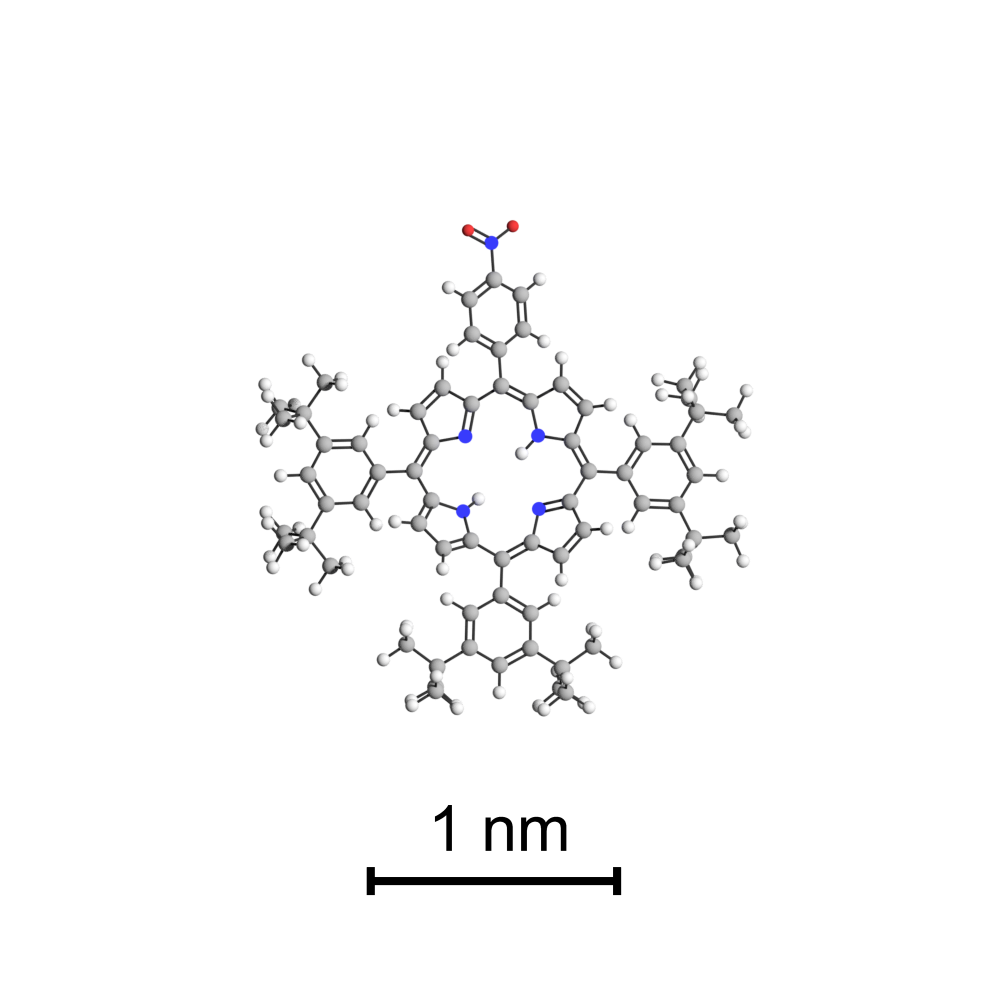
\includegraphics[width=0.45\textwidth]{./images/molecules/TBP-single-scalebar}
		\label{fig:TBP-single}
	} %
	\subfigure[Trans-configuration]{
		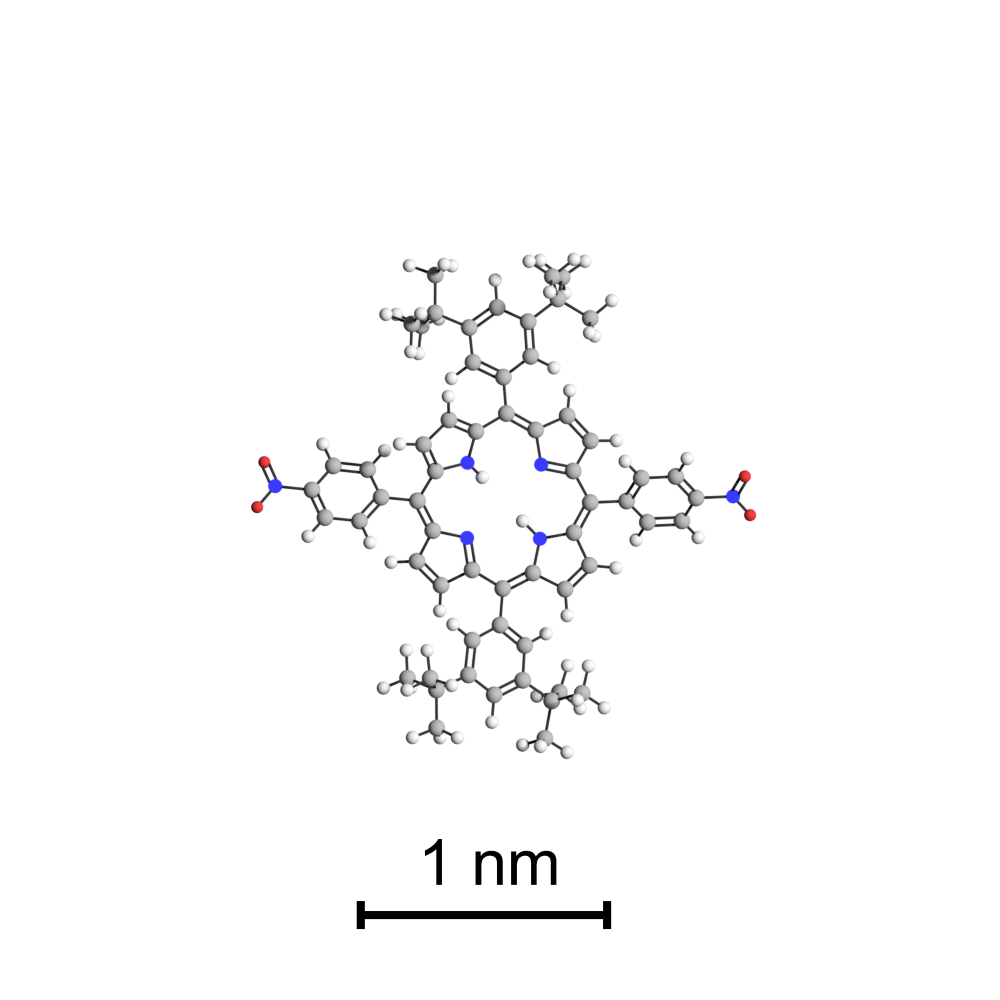
\includegraphics[angle=0, width=0.45\textwidth]{./images/molecules/TBP-trans-scalebar}
		\label{fig:TBP-trans}
	} %
%	\subfigure[Cis-configuration]{
%		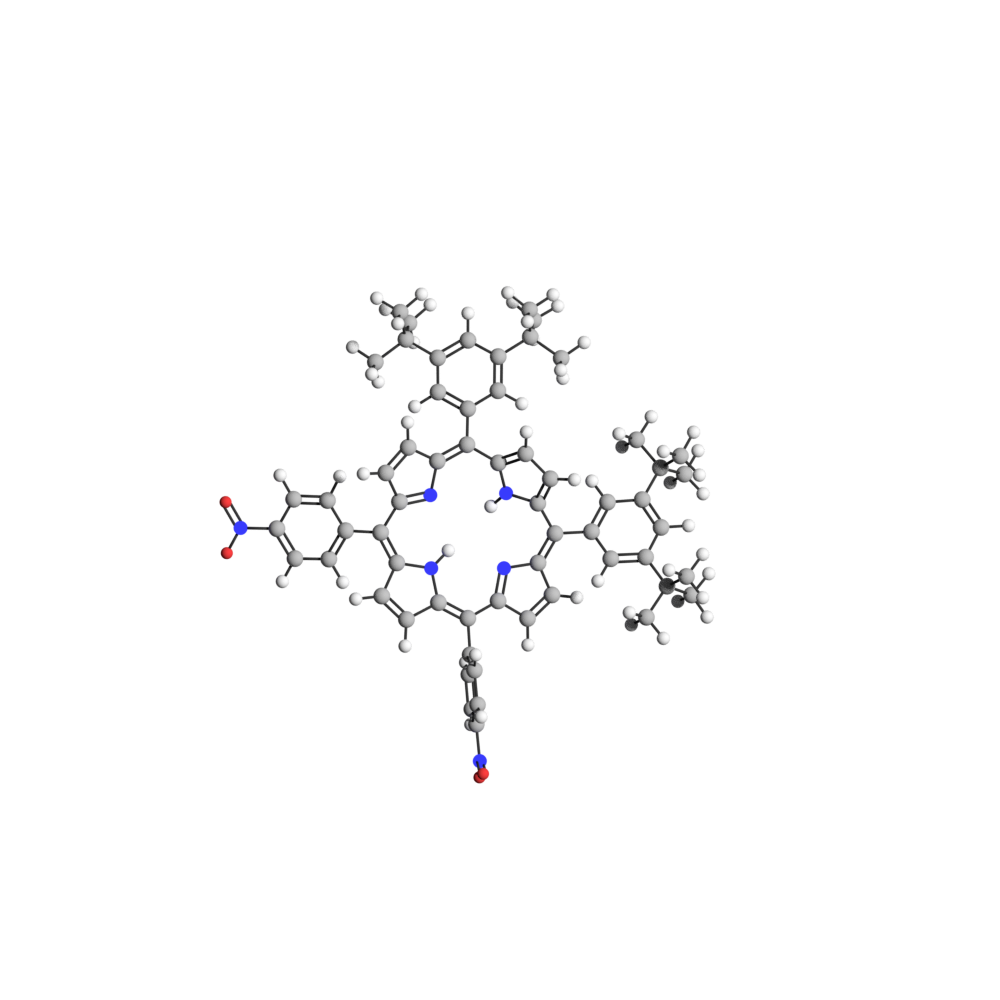
\includegraphics[angle=0, width=0.3\textwidth]{./images/molecules/TBP-cis}
%		\label{fig:TBP-cis}
%	} %
	\caption{Functionalized tert-butyl-phenyl-porphines. \subref{fig:TBP-single} shows a single functionalized porphine molecules. An additional function may be added in %\subref{fig:TBP-cis} cis-  and 
	trans- \subref{fig:TBP-trans} position.}
	\label{fig:TBP}
\end{figure}	

\begin{itemize}
	\item Free base nitrophenyl - 5,10,15 Tri [di-[tert-butyl]-phenyl)]-porphyrin \index{nitro porphin} has 3(2) di-tert-butyl-phenyl groups attached to the porphine macro cycle at the meso-positions of the molecule. The free meso-positions are occupied with nitrophenyl groups as shown in \autoref{fig:TBP-single} If more than one functional group is present, one can distinguish between trans (\autoref{fig:TBP-trans}) and cis configuration (\autoref{fig:TBP-cis}), whether the two functional groups are opposite or neighboring.
	\item The appearance of STM data is correlated to the molecular configuration according to \cite{mishra_current-driven_2015} meaning that the lobes consisting of (3,5-di-tert-butylphenyl) are imaged as bright protrusions, while the functional nitro group is imaged fainter. This holds true for cis- and trans-substituted molecules\cite{yokoyama_selective_2001}.
	\item Tert-butyl groups can rotate to form flexible legs. Interaction with the substrate results in adsorption-induced conformational changes.\cite{ecija_dynamics_2016}
\end{itemize}
Drawings for various functional groups and molecules can be found in \cite{jorgensen_salem_1973}.

\section{Results: Single leg functionalization}
	\subsection{on Cu(111)}
	% TBP on Cu(111)
	\label{sec:single-TBP-Cu111}
	\begin{wrapfigure}{r}{5cm}\centering
		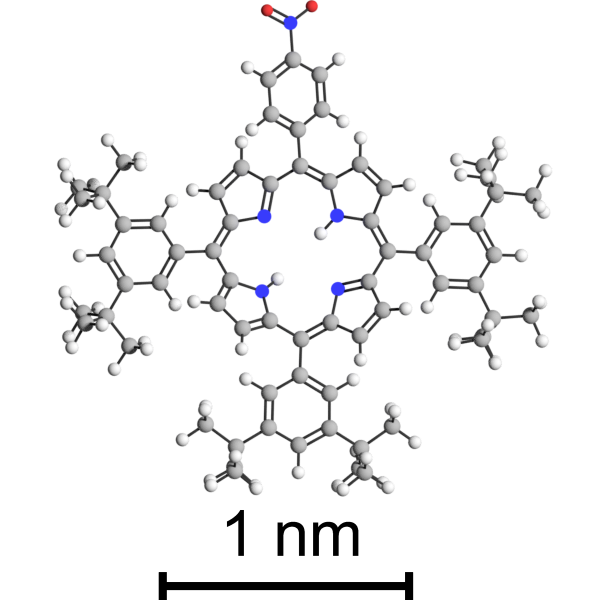
\includegraphics[width=5cm]{./images/molecules/max-zoom/TBP-single-600-scalebar}
		\caption{TBP with three di-tert-butyl and a single nitro phenyl group added at the meso position.}
		\label{fig:}
	\end{wrapfigure}
	When adsorbed at room temperature, TBP distributes equally on the surface, forms unordered islands and decorates step edges. Molecules orient their main axis (connecting line from one di-tert-buytl-phenyl ring across the center to the nitrophenyl ring) along the dense packed substrate rows most often, less are \SI{15}{\degree} of \textcolor{red}{\textbf{((Refer to image?))}}. Several binding motifs (as shown in \autoref{fig:binding-motifs-TBP-Cu111}) are observed, namely
	\begin{itemize}
		\item A dimer, where molecules lie ``head-to-head'', functional groups ($NO_2$) pointing at each other
		\item A ``triangle'', where molecules are rotated \SI{120}{\degree} and functional groups point towards a shared center. Although this motif does not occur very often (or at least under very flexible angles), it is given as an example where the functional groups point to each other. Similar motifs (like 3 molecules in \SI{90}{\degree} are observed together with other orientations. 
		\item Chains with different length appear, where the nitro group of molecule 1 points to the di-tert-butyl group of molecule 2 (``head-to-tail''). At the connection points, molecules appear brighter, promoting a physical overlap of the two molecules.
	\end{itemize}
	
	Center-center distances are typically \SI{1.78}{\nano \meter} (for the head-to-tail) and \SI{1.5}{\nano \meter} for the head-to-head connection. 
	
	\begin{figure}[]
		\centering
		\subfigure[Overview image]{
			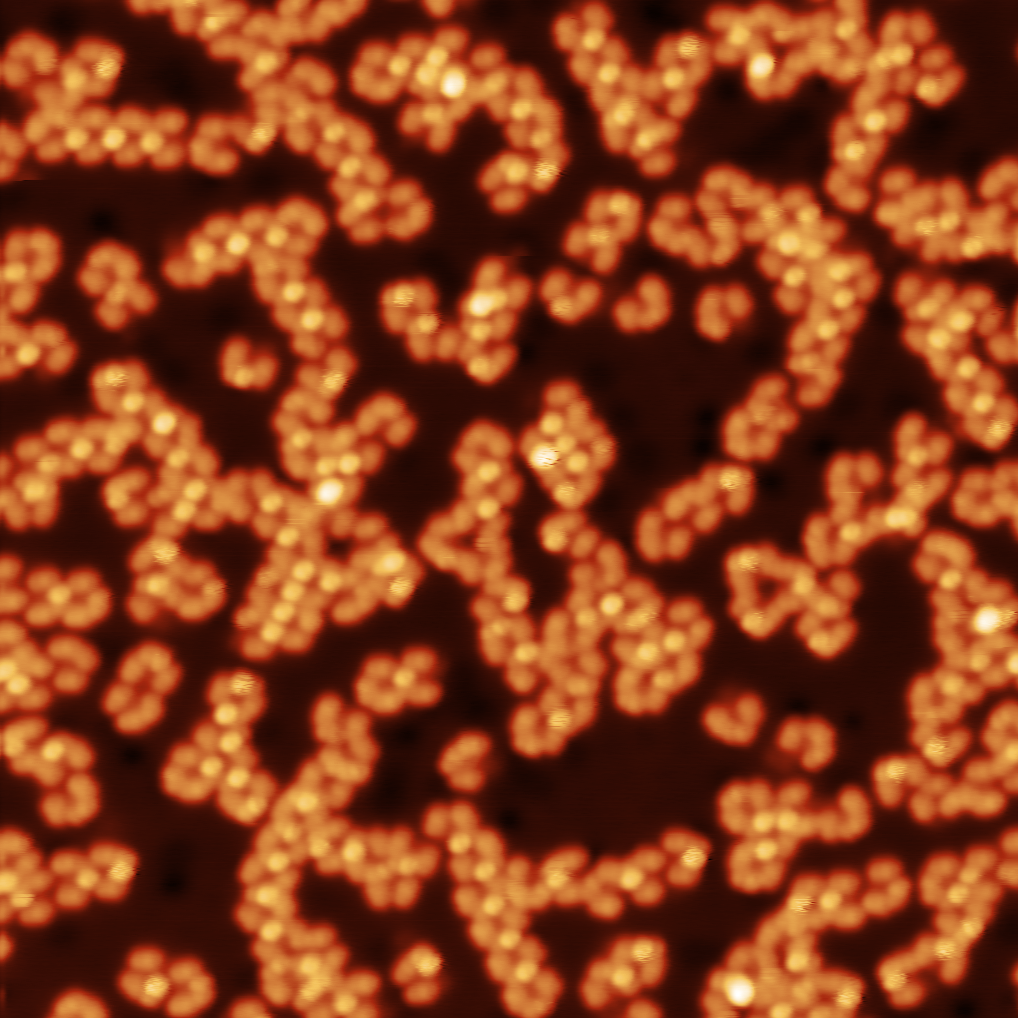
\includegraphics[width=0.7\textwidth]{./images/F151128-083339-44nm}
			\label{fig:single-TBP-cu111-overview}
		}
		
		\subfigure[Monomer]{
			
\includegraphics[width=0.22\textwidth]{./images/F151128-083339-monomer-3nm.png}
			\label{fig:single-TBP-cu111-monomer}	
		}
		\subfigure[Chain]{
			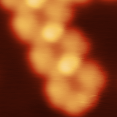
\includegraphics[width=0.22\textwidth]{./images/F151128-083339-chain-5nm}
			\label{fig:single-TBP-cu111-chain}	
		}
		\subfigure[Dimer]{
			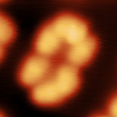
\includegraphics[width=0.22\textwidth]{./images/F151128-083339-dimer-5nm.png}
			\label{fig:single-TBP-cu111-dimer}	
		}
		% \subfigure[Model representation of the binding motifs. See text for more details.]{
		%  \includegraphics[width=0.4\textwidth]{./images/TBP-motivs-on-Cu111}
		% }
		\caption{RT adsorbed single nitro functionalized TBP on Cu(111) and their most abundant binding motifs. \subref{fig:single-TBP-cu111-overview} Each of the binding motif can be found as well in the overview STM data, as well as in the enlarged images (b-d). All images recorded with \SI{-500}{\milli\volt}, \SI{0.1}{\nano\ampere}, color scale \SIrange{0}{300}{\pico\meter}. Image width: \subref{fig:single-TBP-cu111-overview} \SI{44}{\nano\meter}, 
			\subref{fig:single-TBP-cu111-monomer} \SI{3}{\nano\meter}, 	
			\subref{fig:single-TBP-cu111-chain} \& 
			\subref{fig:single-TBP-cu111-dimer} \SI{5}{\nano\meter}
		}
		\label{fig:binding-motifs-TBP-Cu111}
	\end{figure}
	
	\paragraph{``head-to-head''}
	To model the occurring binding motifs, deformations of the molecules have to be taken into account. Because nitro groups face each other in the ``head-to-head'' connection, their distance would be to small to facilitate a similar binding mechanism like for the TPCN on copper (where copper surface ad atoms promote binding between nitrogens), so no free space between the facing nitro groups is observed. Because the distance is so small, the phenyl ring (with attached nitro group) rotates by \SI{45}{\degree}, to make the phenyl ring stand upright. When the second molecule does the same, both match each other with negligible lateral shift, reproducing the STM images best. Similar binding motivs are reported in \cite{kato_dispersive_2008} for non-covalent cross linking of dicarboxylic acids in hydrogels. Although the situation on a metal-surface may change considerably (only 2D - no 3D, metal present - will change chemistry), the observed binding motif matches very well.
	
	\paragraph{``head-to-tail''}
	The chain motif ``head-to-tail'' is reconstructed using the unique contrast of the TBP molecule. When the center-center distance is measured, molecules are modeled that distance away from each other. These models show a physical overlap between molecules, which in not possible because of steric hindrance. To solve the problem, the nitro-group (head) of one molecule if rotated by \SI{35}{\degree} out of the plane (like pulling the nitro-group upwards, not rotating the group left/right). 
	
	%---------------- models bauen und bsp bilder einf\"ugen.  ---------------- 
	
	\paragraph{Flexible tert-butyl-groups}
	\begin{figure}\centering
		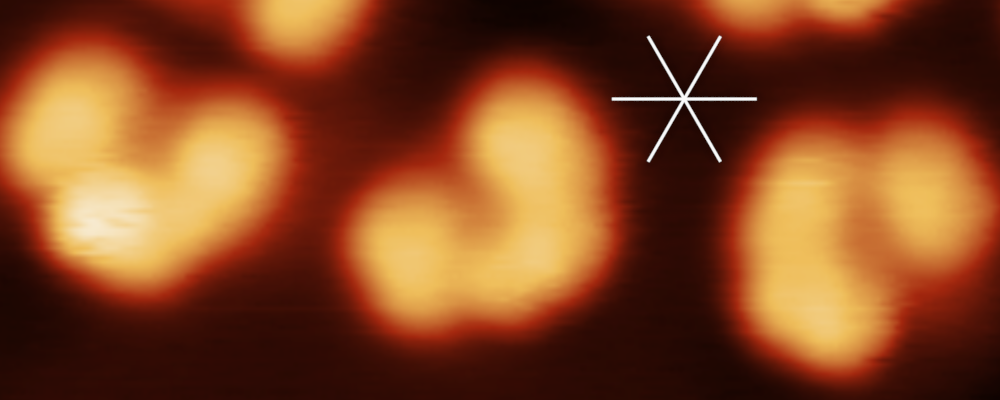
\includegraphics[width=0.44\textwidth]{./images/F151128-083339-10x4-overlay.png}
		\caption{Different appearances of TBP on Cu(111). While most of monomers (center in image above) show even heights with their tert-butyl functions, some (left) do posses an elevated tert-butyl group. The orientation of the tert-butyl groups is aligned with the high symmetry crystal direction (indicated by white lines) most often. Image recorded with  \SI{-500}{\milli\volt}, \SI{0.1}{\nano\ampere}. Image width: \SI{10}{\nano \meter}}
		\label{fig:TPB-butyl-flexibility-SMT}
	\end{figure}
	
	Another interesting fact is that butyl groups of TBP seem to orient them self (as far as steric hindrance allows for) along the dense packed rows of the copper substrate. Again, one has to be careful when reconstructing geometrical information from STM images. Like the distortion of legs in the TPCN molecule, this rotation can be explained by a rotation of single butyl groups. Although the phenyl ring remains at the same position/rotation, tert-butyl groups are allowed to rotate such that they appear in different heights. Because STM (constant current) follows equipotential lines, the whole phenyl-di-tert-butyl-complex looks rotated in plane, although it may not be. This is confirmed in literature\cite{heim_surface-assisted_2010, heim_self-assembly_2010}.
	
	%%%%%%%%%%%%%%%%%%%%%%%%%%%%%%%%%%%%%%%%%%%%%%%%%%%%%%%%%%%%%%%%%%%%%%%%%%%%%%%%%%
	\subsection{on Ag(111)}
	% This is TBP on Ag(100):
	\label{sec:single-TBP-Ag100}
	%%%%%%%%%%%%%%%%%%%%%%%%%%%%%%%%%%%%%%%%%%%%%%%%%%%%%%%%%
	Molecules are adsorbed on Ag(100) at RT. The resulting conglomerates are shown in \autoref{fig:single-TBP-Ag100-RT}. The very most surface area is covered with unregular patterns. The step edges are covered, assuming a sufficient large mobility at RT to move from the terrace to the nearest step edge. The only free step edges observed are due to tip formings on the sample surface since these are created after the molecules are stuck on the surface because of the low temperatures during measurement.
	%%%%%%%%%%%%%%%%%%%%%%%%%% Annealing %%%%%%%%%%%%%%%%%%%%%%%%%%%%%%%%%%%%%
	\paragraph{Annealing}
	The RT adsorption is annealed to \SI{170}{\celsius} for \SI{10}{\min} and investigated in LT-STM again (\autoref{fig:single-TBP-Ag100-annealed}). No big changes are visible, neither in the formation of new assemblies nor in the distribution of molecules at terraces or at step edges. No chain formation could be observed.
	
	\begin{figure}[] \centering
		\subfigure[Adsorption at RT]{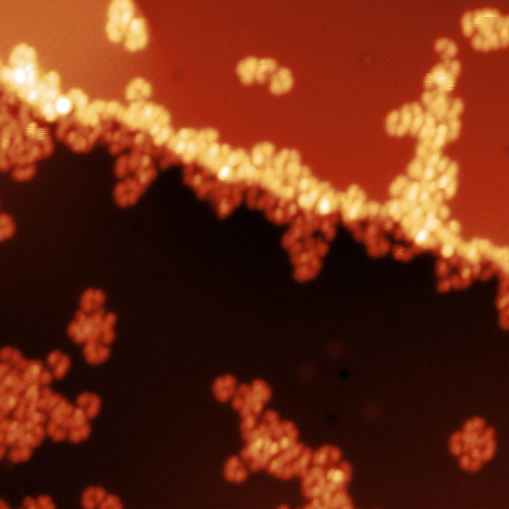
\includegraphics[width=0.45\textwidth]{./images/F150615-121334-cut.png}
			\label{fig:single-TBP-Ag100-RT}
		}
		\subfigure[RT adsorption annealed to \SI{170}{\celsius} for \SI{10}{\min}]{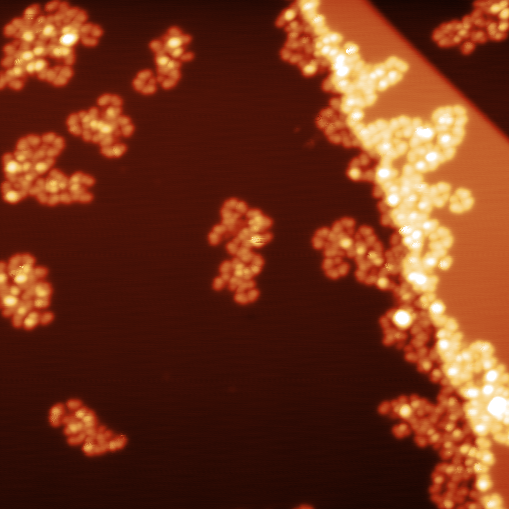
\includegraphics[width=0.45\textwidth]{./images/F150616-102758-44nm.png}
			\label{fig:single-TBP-Ag100-annealed}
		}
		\caption{Annealing after RT adsorption of molecules on Ag(100). \subref{fig:single-TBP-Ag100-RT} STM data of molecules adsorbed at RT (Scan parameters: $U_b=\SI{1}{\volt}, I_t=\SI{0,03}{\nano \ampere}$), \subref{fig:single-TBP-Ag100-annealed} After annealing for \SI{10}{\min} to \SI{170}{\celsius} (Scan parameters: $U_b=\SI{1}{\volt}, I_t=\SI{0,1}{\nano \ampere}$). Color scale \SIrange{0}{600}{\pico\meter}. Image width: \SI{44}{\nm}.}
		\label{fig:single-TBP-Ag100-annealing}
	\end{figure}
	
	%%%%%%%%%%%%%%%%%%%%%%%%%% Assembly models %%%%%%%%%%%%%%%%%%%%%%%%%%%%%%%%%%%%%
	\paragraph{Assembly}
	Since no regular self-assembled islands are present on the surface, more detail is put on the only repeating binding motifs on this surface. One of this configurations resembles a cross (\autoref{fig:single-TBP-Ag100-cross}), while the second one is a variation of the dimer motif (\autoref{fig:single-TBP-Ag100-doubledimer}).
	
	%%%%%%%%%%%%%%%%%%%%%%%% Dimer %%%%%%%%%%%%%%%%%%%%%%%%%%%%%%%%
	
	While on copper, two molecules may form a dimer in head-to-head of head-to-tail configuration, on silver some form tetramers from two parallel merged dimers. While one dimer looks like two ``U'''s with facing open ends ($\in \ni$), the other dimer is shifted to closely match the first dimer best and lies parallel.
	
	%\begin{figure}[] \centering
	%
	%	\caption{Dimer configuration of TBP adsorbed on Ag(100) at RT. \subref{fig:single-TBP-Ag100-dimer} STM data. Scan parameters: $U_b=\SI{0.328}{\volt}, I_t=\SI{0.035}{\nano \ampere}$, color scale \SIrange{0}{300}{\pico\meter}. Image width: \SI{5}{\nm}. \subref{fig:single-TBP-Ag100-dimer-model} Model representation in the same size.}
	%	\label{fig:single-TBP-Ag100-dimer}
	%\end{figure}
	
	%%%%%%%%%%%%%%%%%%%%%%%% Double Dimer %%%%%%%%%%%%%%%%%%%%%%%%%%%%%%%%
	\begin{figure}[] \centering
		\subfigure[]{  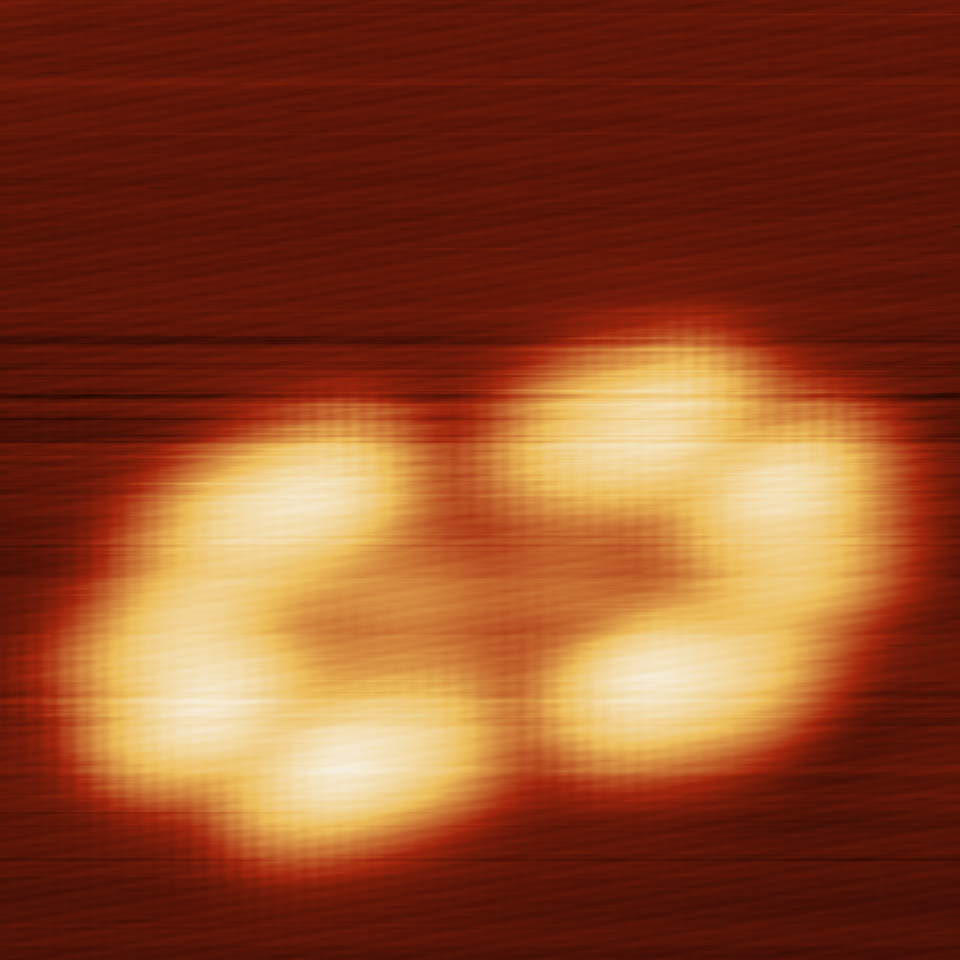
\includegraphics[width=0.3\textwidth]{./images/F150612-153409-5nm.png}
			\label{fig:single-TBP-Ag100-dimer-STM}
		}
		\subfigure[]{  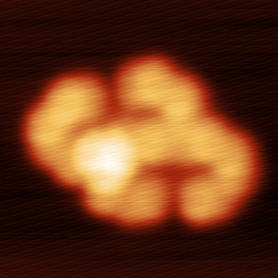
\includegraphics[width=0.3\textwidth]{./images/F150612-144915-6nm.png}
			\label{fig:single-TBP-Ag100-doubledimer-STM}
		}
		\subfigure[]{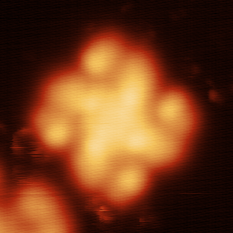
\includegraphics[width=0.3\textwidth]{./images/F150612-154558-10nm.png}
			\label{fig:single-TBP-Ag100-cross-STM}
		}
		\subfigure[]{  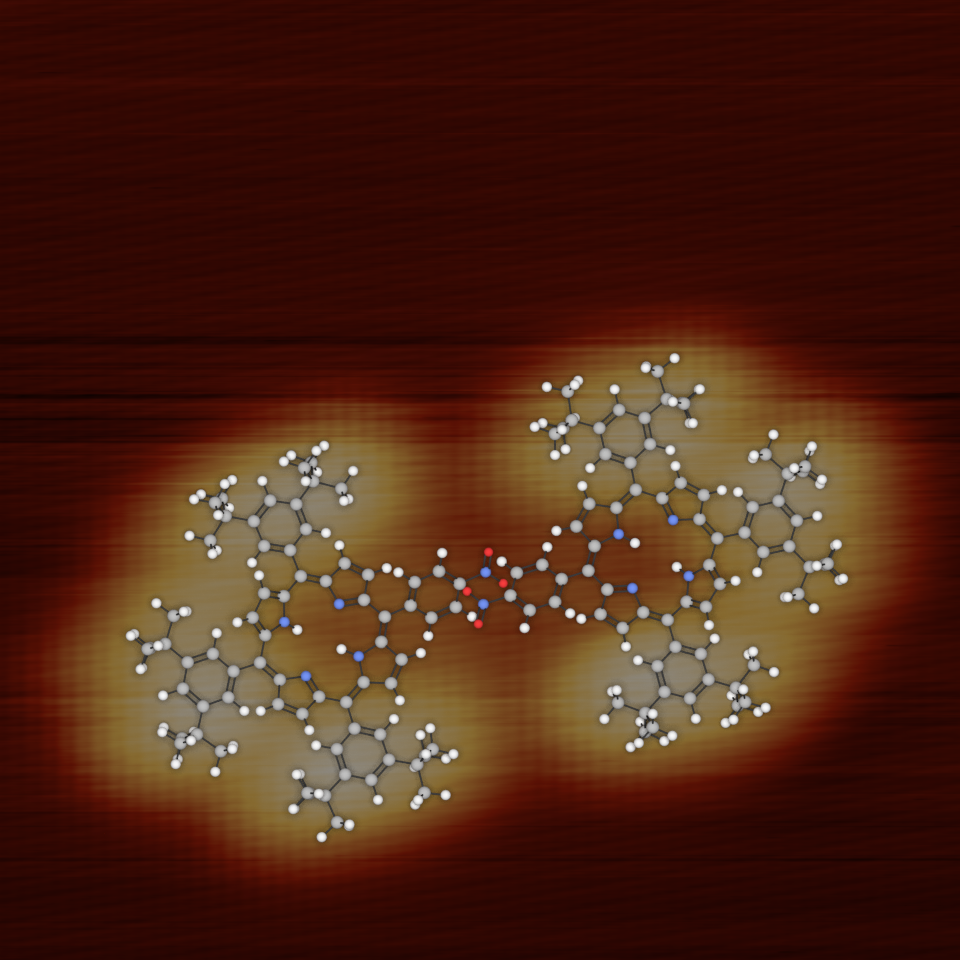
\includegraphics[width=0.3\textwidth]{./images/F150612-153409-5nm-model.png}
			\label{fig:single-TBP-Ag100-dimer-model}
		}
		\subfigure[]{  \includegraphics[width=0.3\textwidth]{./images/F150612-144915-6nm-model}
			\label{fig:single-TBP-Ag100-doubledimer-model}
		}
		\subfigure[]{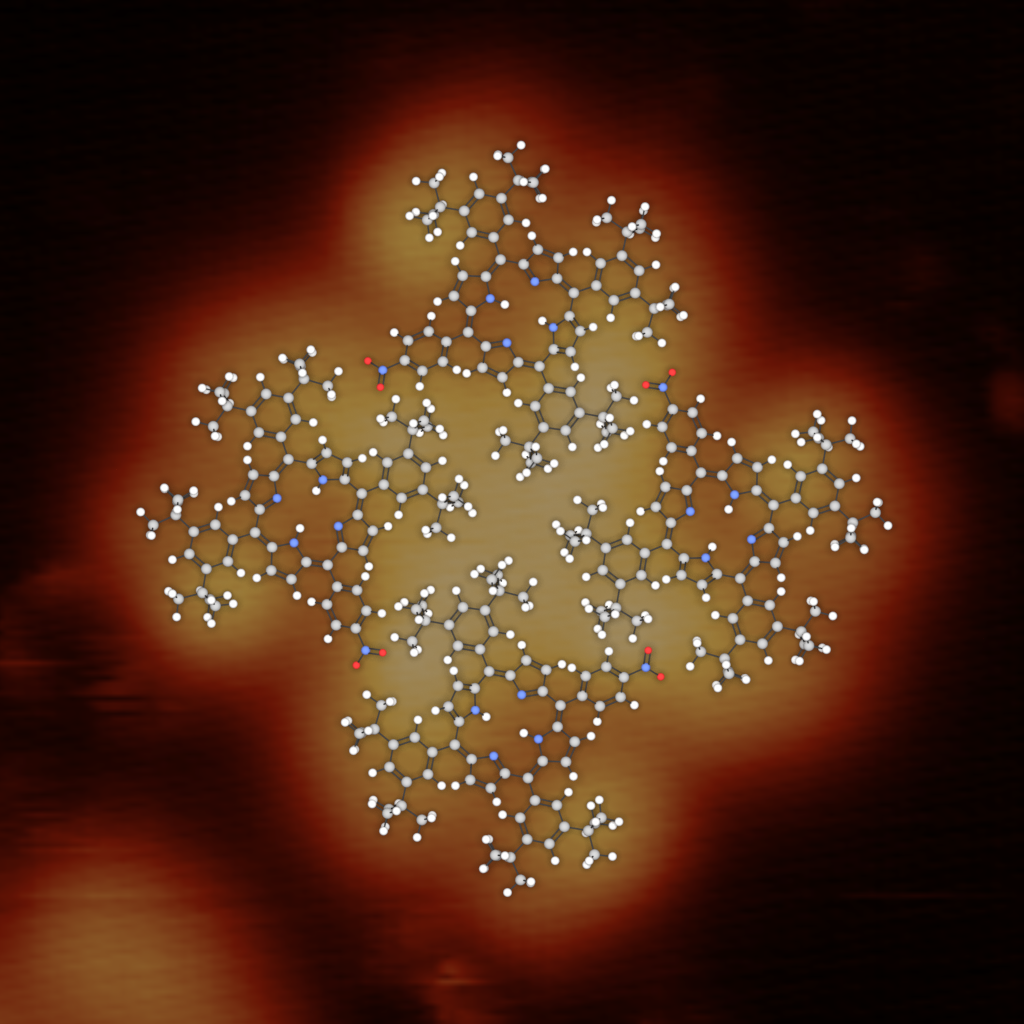
\includegraphics[width=0.3\textwidth]{./images/F150612-154558-10nm-model3.png}
			\label{fig:single-TBP-Ag100-cross-model}
		}
		\caption{Different observed binding configurations of TBP adsorbed on Ag(100) at RT. \subref{fig:single-TBP-Ag100-dimer-STM} STM data of dimer configuration. Scan parameters: $U_b=\SI{0.328}{\volt}, I_t=\SI{0.035}{\nano \ampere}$, Image width: \SI{5}{\nm}. \subref{fig:single-TBP-Ag100-dimer-model} Model representation. \subref{fig:single-TBP-Ag100-doubledimer-STM} STM data of two coalescent dimers. Scan parameters: $U_b=\SI{0.097}{\volt}, I_t=\SI{0.035}{\nano \ampere}$, Image width: \SI{6}{\nm}. \subref{fig:single-TBP-Ag100-doubledimer-model} Model representation. \subref{fig:single-TBP-Ag100-cross-STM} A cross consisting of four TBP molecules. Scan parameters: $U_b=\SI{2.3}{\volt}, I_t=\SI{0,035}{\nano \ampere}$, Image width: \SI{10}{\nm}. \subref{fig:single-TBP-Ag100-cross-model} Model representation. Color scale in all STM images \SIrange{0}{300}{\pico\meter}}
		\label{fig:single-TBP-Ag100-doubledimer}
	\end{figure}
	%%%%%%%%%%%%%%%%%%%%%%%% Cross %%%%%%%%%%%%%%%%%%%%%%%%%%%%%%%%
	Another motif looks like a cross and shown in \autoref{fig:single-TBP-Ag100-cross-model}. Build out of four molecules, where each is rotated by \SI{90}{\degree} with respect to its preliminary neighbor. One can distinguish four di-tert-butyl groups from the central cross. Although there is no atom directly in the center, the cross looks bright in its center (in STM), which is somehow counterintuitive. 
	
	%\begin{figure}[] \centering
	%
	%	\caption{\subref{fig:single-TBP-Ag100-cross-STM} A cross consisting of four TBP molecules. Scan parameters: $U_b=\SI{2.3}{\volt}, I_t=\SI{0,035}{\nano \ampere}$, color scale \SIrange{0}{300}{\pico\meter}. Image width: \SI{10}{\nm}. \subref{fig:single-TBP-Ag100-cross-model} Model representation in the same size.}
	%	\label{fig:single-TBP-Ag100-cross}
	%\end{figure}
	
	\paragraph{Flexible Tert-Butyl-Functions}
	\autoref{fig:single-TBP-Ag100-doubledimer-STM} shows an interesting feature of the tert-butyl functions.
	
	\begin{itemize}
		\item Butyl groups within TBP feature different contrasts (look rotated), while the orientation of the butyl-groups doesn't follow the close packed substrate rows. ---------------- find image and explain
		\item TBP molecules have been heated on silver substrate for \SI{10}{\minute} at \SI{170}{\celsius}. The resulting sample did not feature chain-formation or improved ordering.
	\end{itemize}
	
	%%%%%%%%%%%%%%%%%% Single ordered area => Appendix? %%%%%%%%%%%%%%%%%%%%
	%-------------- Add graphic to explain!-------------- 
	
	%%%%%%%%%%%%%%%%%% Spectra %%%%%%%%%%%%%%%%%%%%
	\paragraph{Spectroscopy}
	\textcolor{red}{\textbf{
			Some spectroscopy could be achieved that shows different typical features for different areas in the molecule. Note that the spectra were done for molecules sitting on a Ag(100) surface.
			There is a clear indication, that the macrocycle of the molecule contributes to the broad peak in the dI/dV data at around \SI{1}{\V}, while the nitro groups dominate the spectra at around \SI{600}{\milli \V}. 
			Look at the corresponding .pptx file for the spectra and the corresponding IGOR-files dimer/quatermer1-2 for the spectra.
		}
	}
	\subsection{on \textit{h}-BN}
	%%%%%%%%%%%%%%%%%%%%%%%%%%%TBP on h-BN/Cu(111)
	\label{section:TBP-on-hBN}
	\begin{figure}[] \centering
		\subfigure[\textit{h}-BN grown on Cu(111).]{
			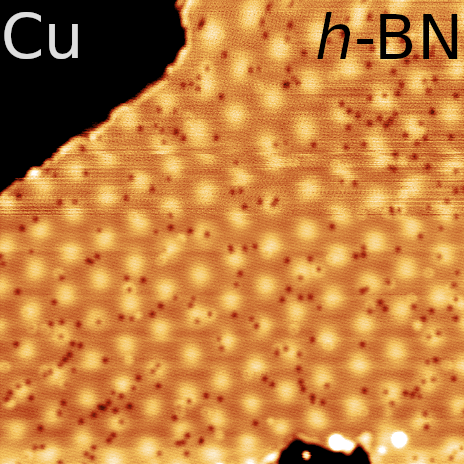
\includegraphics[width=0.3\textwidth]{./images/F151130-135150-40nm-text}
			\label{fig:h-BN-Cu111}
		}
		\subfigure[TBP after adsorption on \textit{h}-BN/Cu(111)]{
			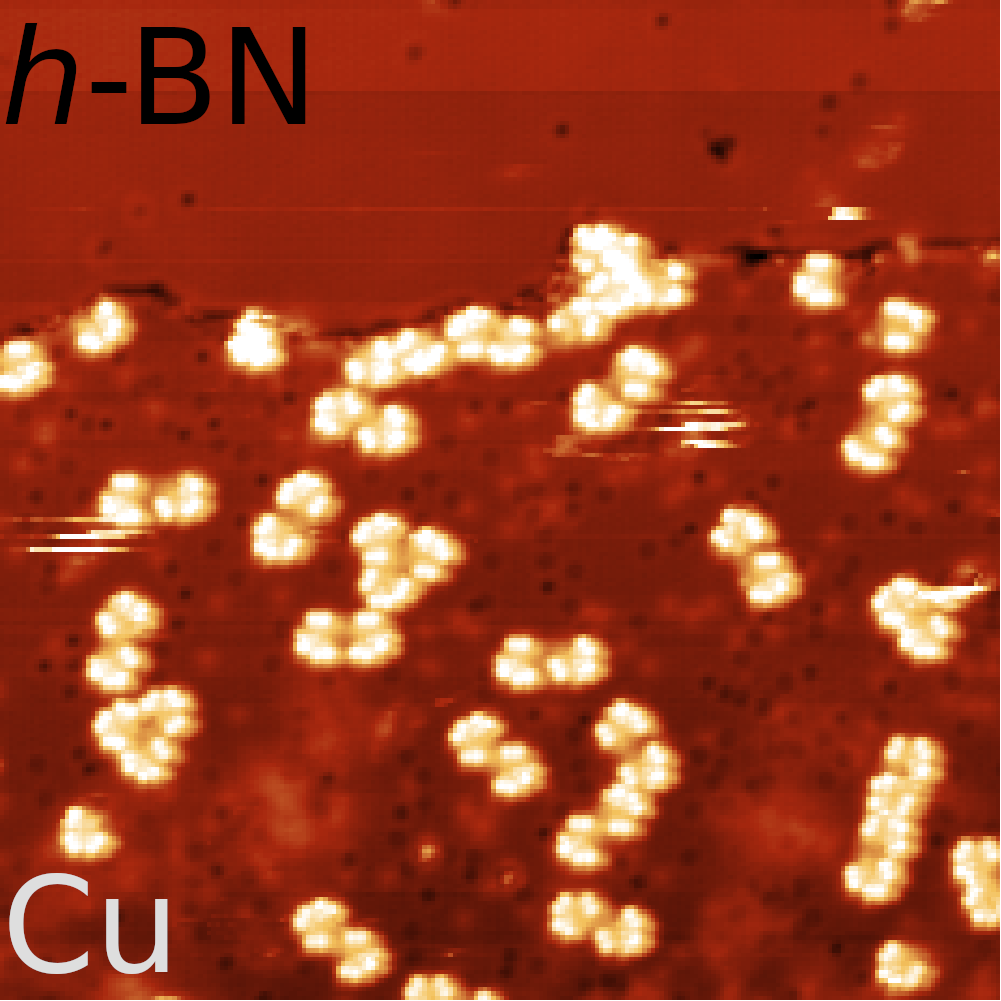
\includegraphics[width=0.3\textwidth]{./images/F160617-110201-40nm-text}
			\label{fig:single-TBP-hBN-cu111}
		}
		\subfigure[TBP after adsorption on \textit{h}-BN/Cu foil.]{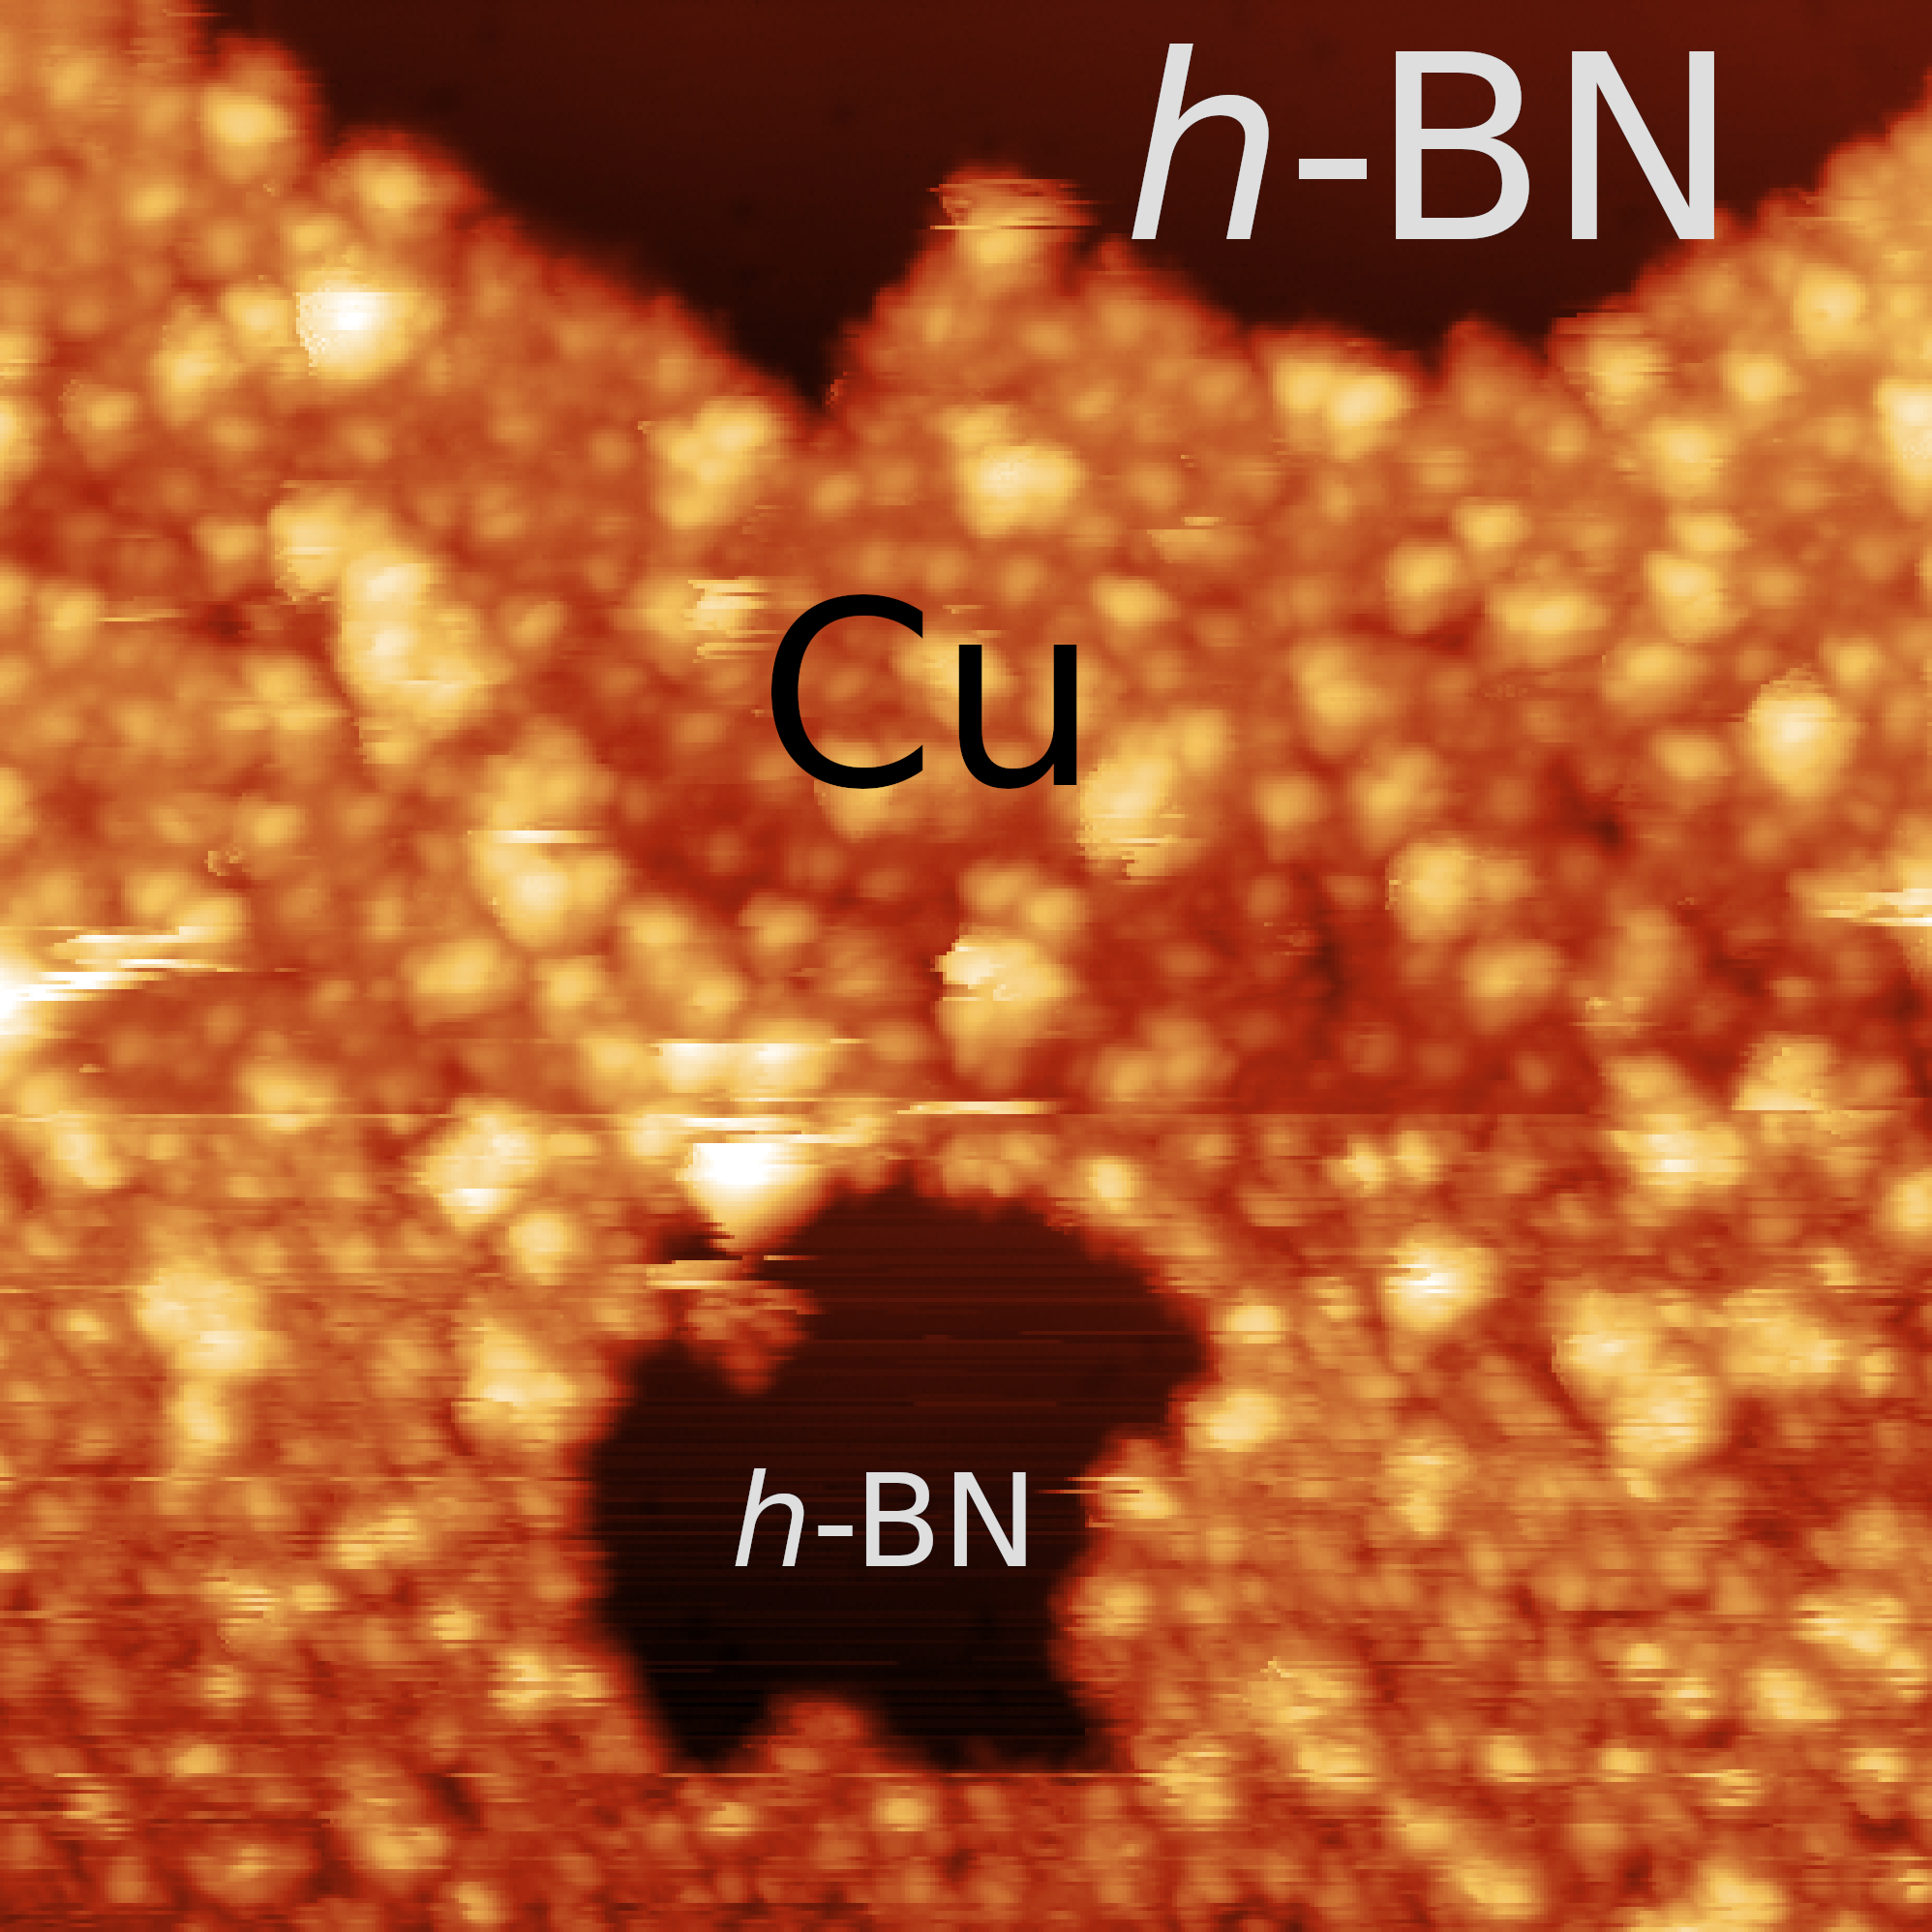
\includegraphics[width=0.3\textwidth]{./images/F151123-110602-40nm-text}
			\label{fig:single-TBP-hBN-cu-foil}
		}
		\caption{STM topographs of \textit{h}-BN grown on copper with subsequent molecular adsorption. \subref{fig:h-BN-Cu111} shows a \textit{h}-BN layer grown on Cu(111) by CVD. \subref{fig:single-TBP-hBN-cu111} shows the sample after evaporating TBP molecules at RT. \subref{fig:single-TBP-hBN-cu-foil} shows empty \textit{h}-BN islands grown on the polycrystalline copper foil and molecules on a copper terrace. 
			Scan parameters: \subref{fig:h-BN-Cu111} $U_b=\SI{2.273}{\volt}, I_t=\SI{0.048}{\nano \ampere}$, color scale \SIrange{0}{100}{\pico \meter}. \subref{fig:single-TBP-hBN-cu111} $U_b=\SI{1.074}{\volt}, I_t=\SI{0.033}{\nano \ampere}$, color scale \SIrange{0}{300}{\pico \meter}. \subref{fig:single-TBP-hBN-cu-foil} $U_b=\SI{2.585}{\volt}, I_t=\SI{0.032}{\nano \ampere}$, color scale \SIrange{0}{1500}{\pico \meter}.  All images are \SI{40}{\nano \meter} wide.}
		\label{TBP-on-hBN}
	\end{figure}
	
	\paragraph{\textit{h}-BN grown on Cu(111)}
	\textcolor{red}{\textbf{
			Further experiments have can done to investigate the behavior of TBP on \textit{h}-BN. When adsorbed on \textit{h}-BN/Cu(111), molecules show a high mobility that makes the molecules move away from the \textit{h}-BN islands. Some molecules could be resolved at defects or close to the perimeter of the \textit{h}-BN islands. This is in line with other observations for adsorbates ((CITATION)). Adsorption temperatures as low as \SI{-170}{\celsius} have been used to lower the molecules' energy pool, but diffusion to free metal areas occurs and no molecules remain on the \textit{h}-BN surface.
		}}
		
		%single-TPB-on-h-bn-cu-foil
		\paragraph{\textit{h}-BN grown on Cu-foil}
		\textcolor{red}{\textbf{
				Molecules adsorb on the BN surface and STM imaging is hard due to molecules that can be moved on the rather 'slippy' surface of the insulating BN. Nevertheless some agglomerations of the molecules leave free BN spots where no molecules are. As the preparation of the BN should result in a closed BN layer on top of the Cu-foil no movement of molecules to free Cu areas should be observed, making these free regions BN regions.
				Why the molecules are not distributed homogenously on the BN remains topic to speculation.
				Spectroscopy has been tried intensively but without reproduceable results.
				Unlike the adsorption on Ag(100) and Cu(111) no formation of di- and quatermers has been observed.
				% See experiments in June '16
			}}

\section{Results: Double leg functionalization}
	\subsection{on Cu(111)}
	% tbp-double on Cu(111)
	\begin{wrapfigure}{r}{5cm}\centering
		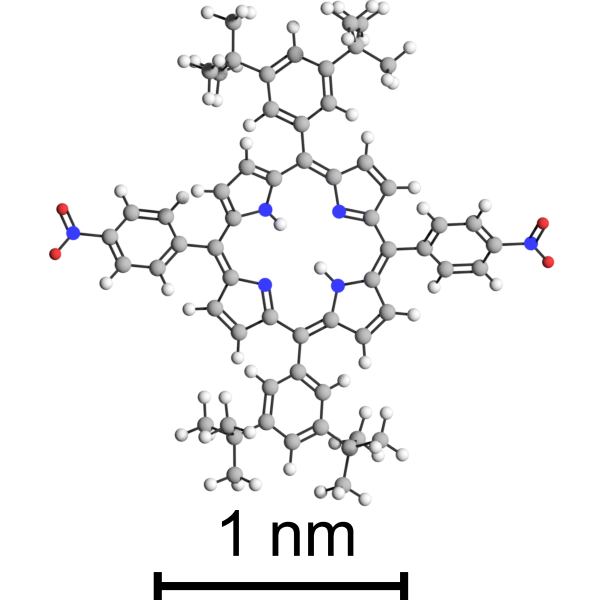
\includegraphics[width=5cm]{./images/molecules/max-zoom/TBP-trans-600-scalebar}
		\caption{}
	\end{wrapfigure}
	
	When depositing trans-TBP on Cu(111) at room temperature no long range ordering can be achieved. The molecules arrange rather arbitrarily as can be seen in  \autoref{fig:two-leg-trans-cu111-rt}.
	
	\begin{figure}[h]
		\centering
		\subfigure[]{
			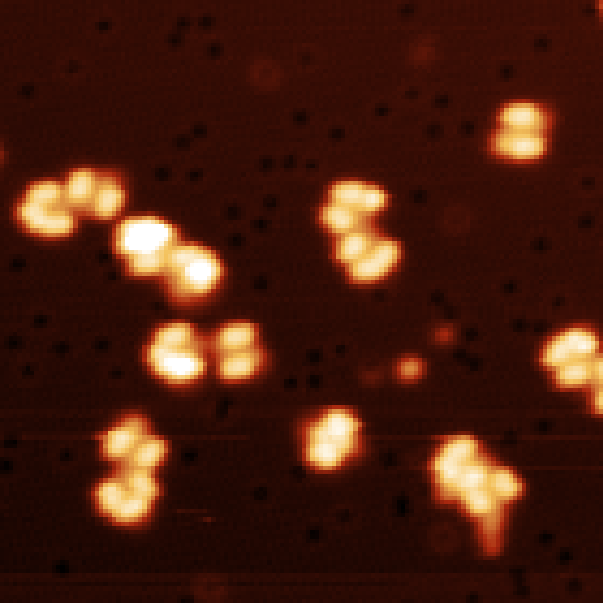
\includegraphics[width=0.3\textwidth]{./images/F160425-172349-40nm}
			%IMAGE SCANNED COARSE!!
			\label{fig:two-leg-trans-cu111-rt}
		}
		\subfigure[New preparation adsorbed at \SI{70}{\celsius}]{
			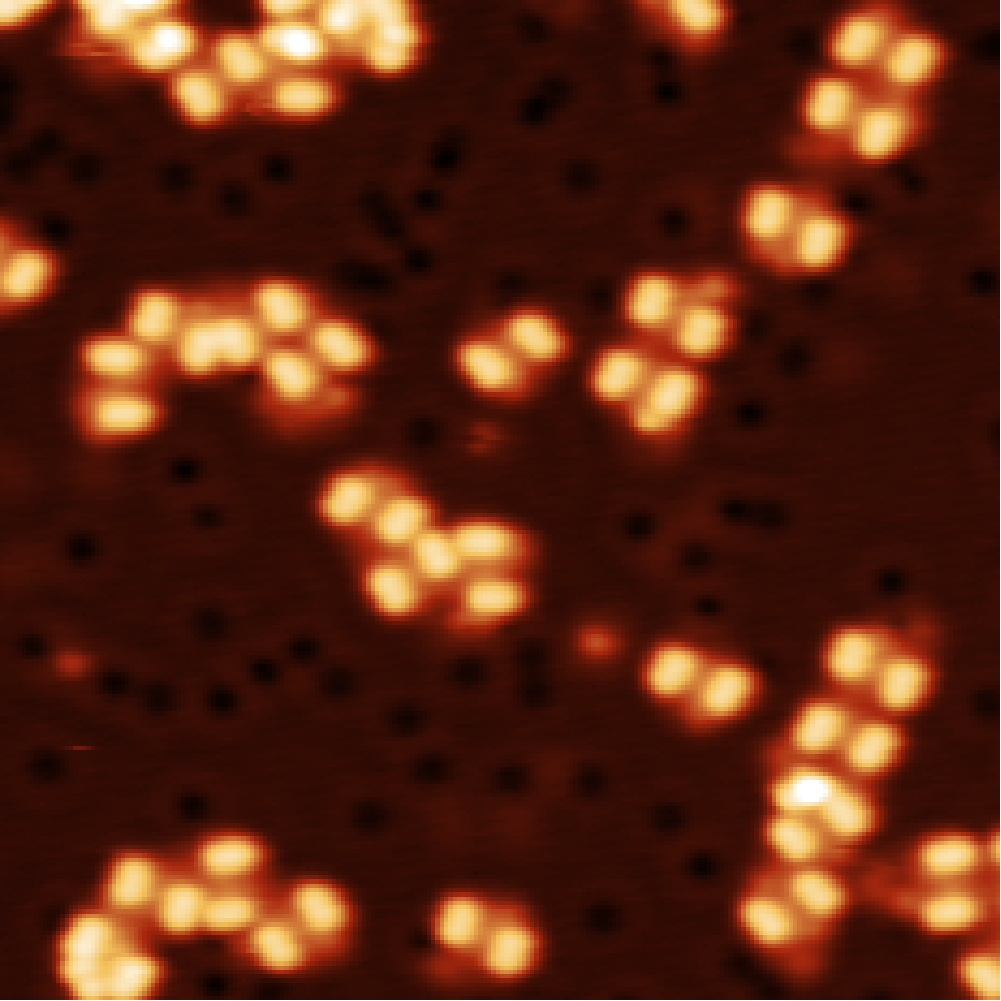
\includegraphics[width=0.3\textwidth]{./images/F160427-121720-40nm}
			\label{fig:two-leg-trans-cu111-70c} 
			%IMAGE SCANNED COARSE!!
		}
		\subfigure[... and heated for \SI{10}{\minute} to \SI{170}{\celsius}]{
			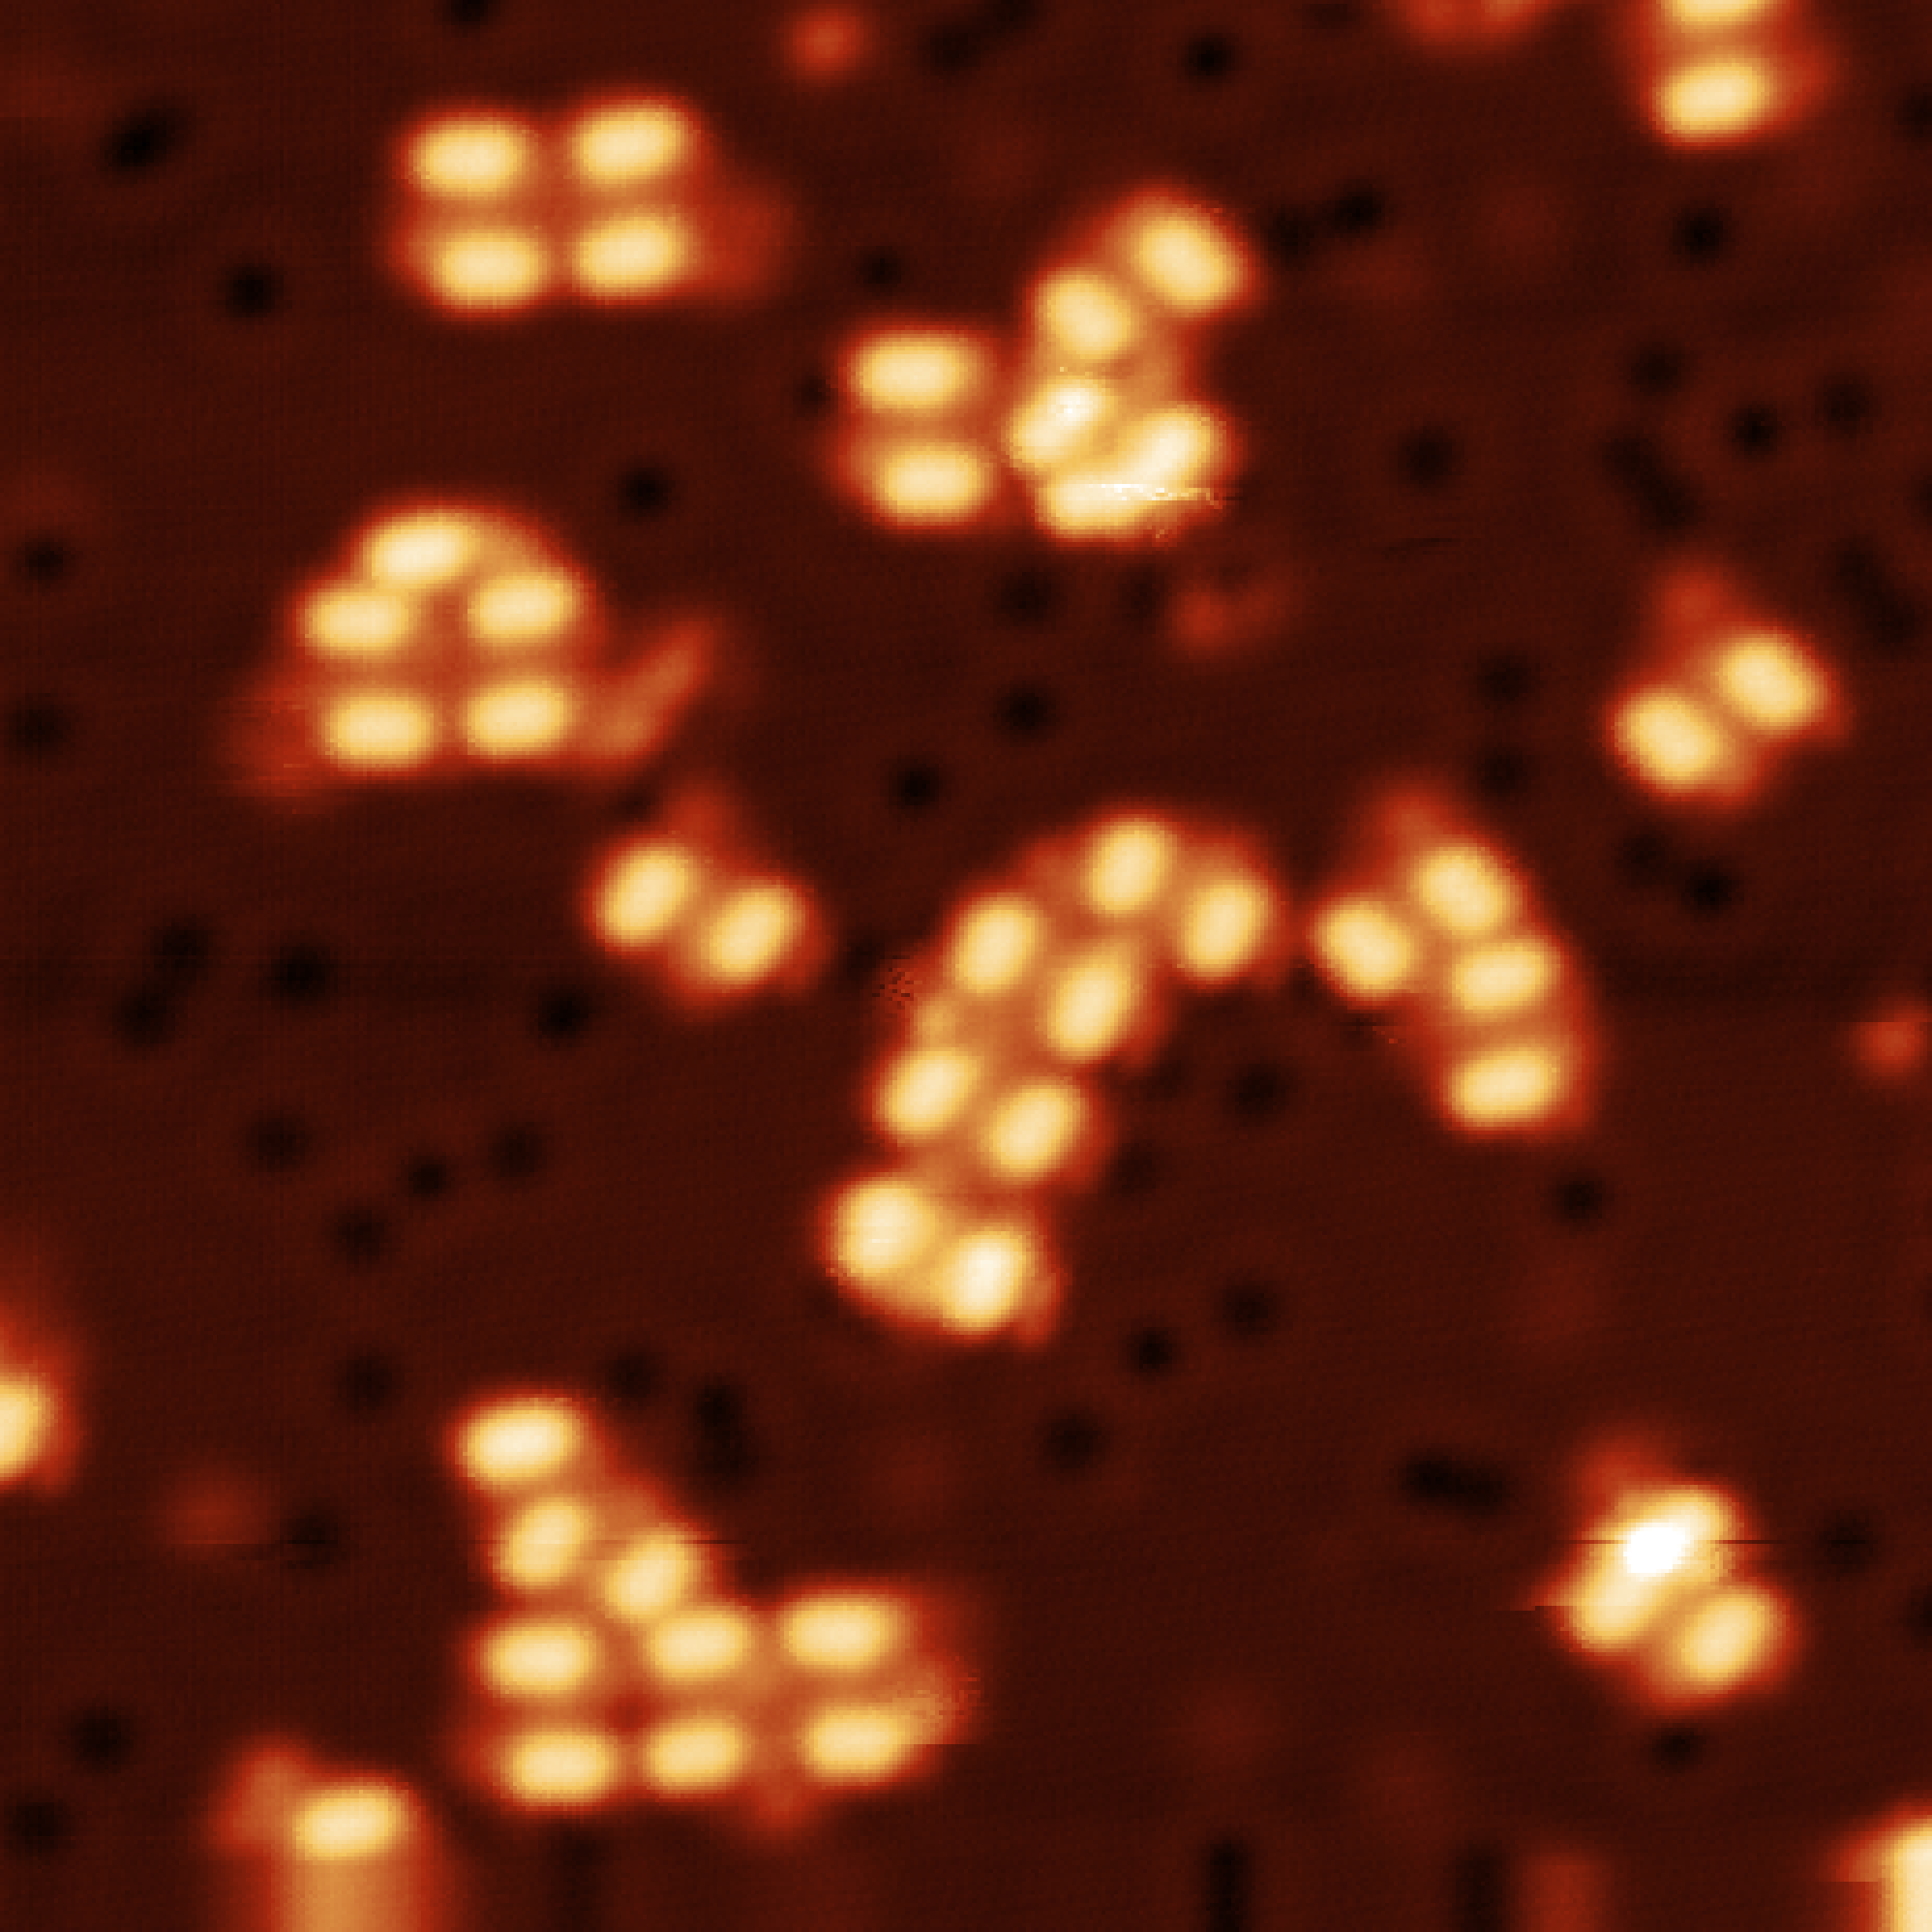
\includegraphics[width=0.3\textwidth]{./images/F160427-142006-40nm}
			\label{fig:two-leg-trans-cu111-170c}
			%IMAGE SCANNED COARSE!!
		}
		\caption{Molecules adsorbed on Cu(111) at RT and subsequently annealed to different temperatures. \subref{fig:two-leg-trans-cu111-rt} Adsorption at room temperature did not show extended long range order. \subref{fig:two-leg-trans-cu111-70c}  Adsorption at \SI{70}{\celsius} and \subref{fig:two-leg-trans-cu111-170c} annealing to \SI{170}{\celsius} for \SI{10}{\minute} improves the chain length slightly. All images are \SI{40}{\nano \meter} wide. Scan parameters: \subref{fig:two-leg-trans-cu111-rt} $U_b=\SI{1.2}{\volt}, I_t=\SI{0.041}{\nano \ampere}$, \subref{fig:two-leg-trans-cu111-70c} $U_b=\SI{0.5}{\volt}, I_t=\SI{0.038}{\nano \ampere}$, \subref{fig:two-leg-trans-cu111-170c} $U_b=\SI{0.522}{\volt}, I_t=\SI{0.021}{\nano \ampere}$}
		\label{fig:two-leg-trans-cu111}
		%ALL OF THE IMAGES SCANNED COARSE!!
	\end{figure}
	
	The molecules tend to connect in a \textbf{\textcolor{red}{defined angle}} to its next neighbor, forming different binding motifs. These are predominantly different kind of chain formation (see figure \ref{fig:two-leg-trans-cu111-motifs}).
	\begin{itemize}
		\item The molecules are ordered such that they form a straight chain (\autoref{trans-nitro-on-cu111-70-straight-chain}).
		\item The molecules arrange in chains, but each molecule has an offset of about a half of its width to the next neighbor or the molecules attach in chains, but show a kink. \autoref{trans-nitro-on-cu111-70-shifted-chain}
	\end{itemize}
	
	\begin{figure}[h]
		\centering
		\subfigure[Straight chain]{
			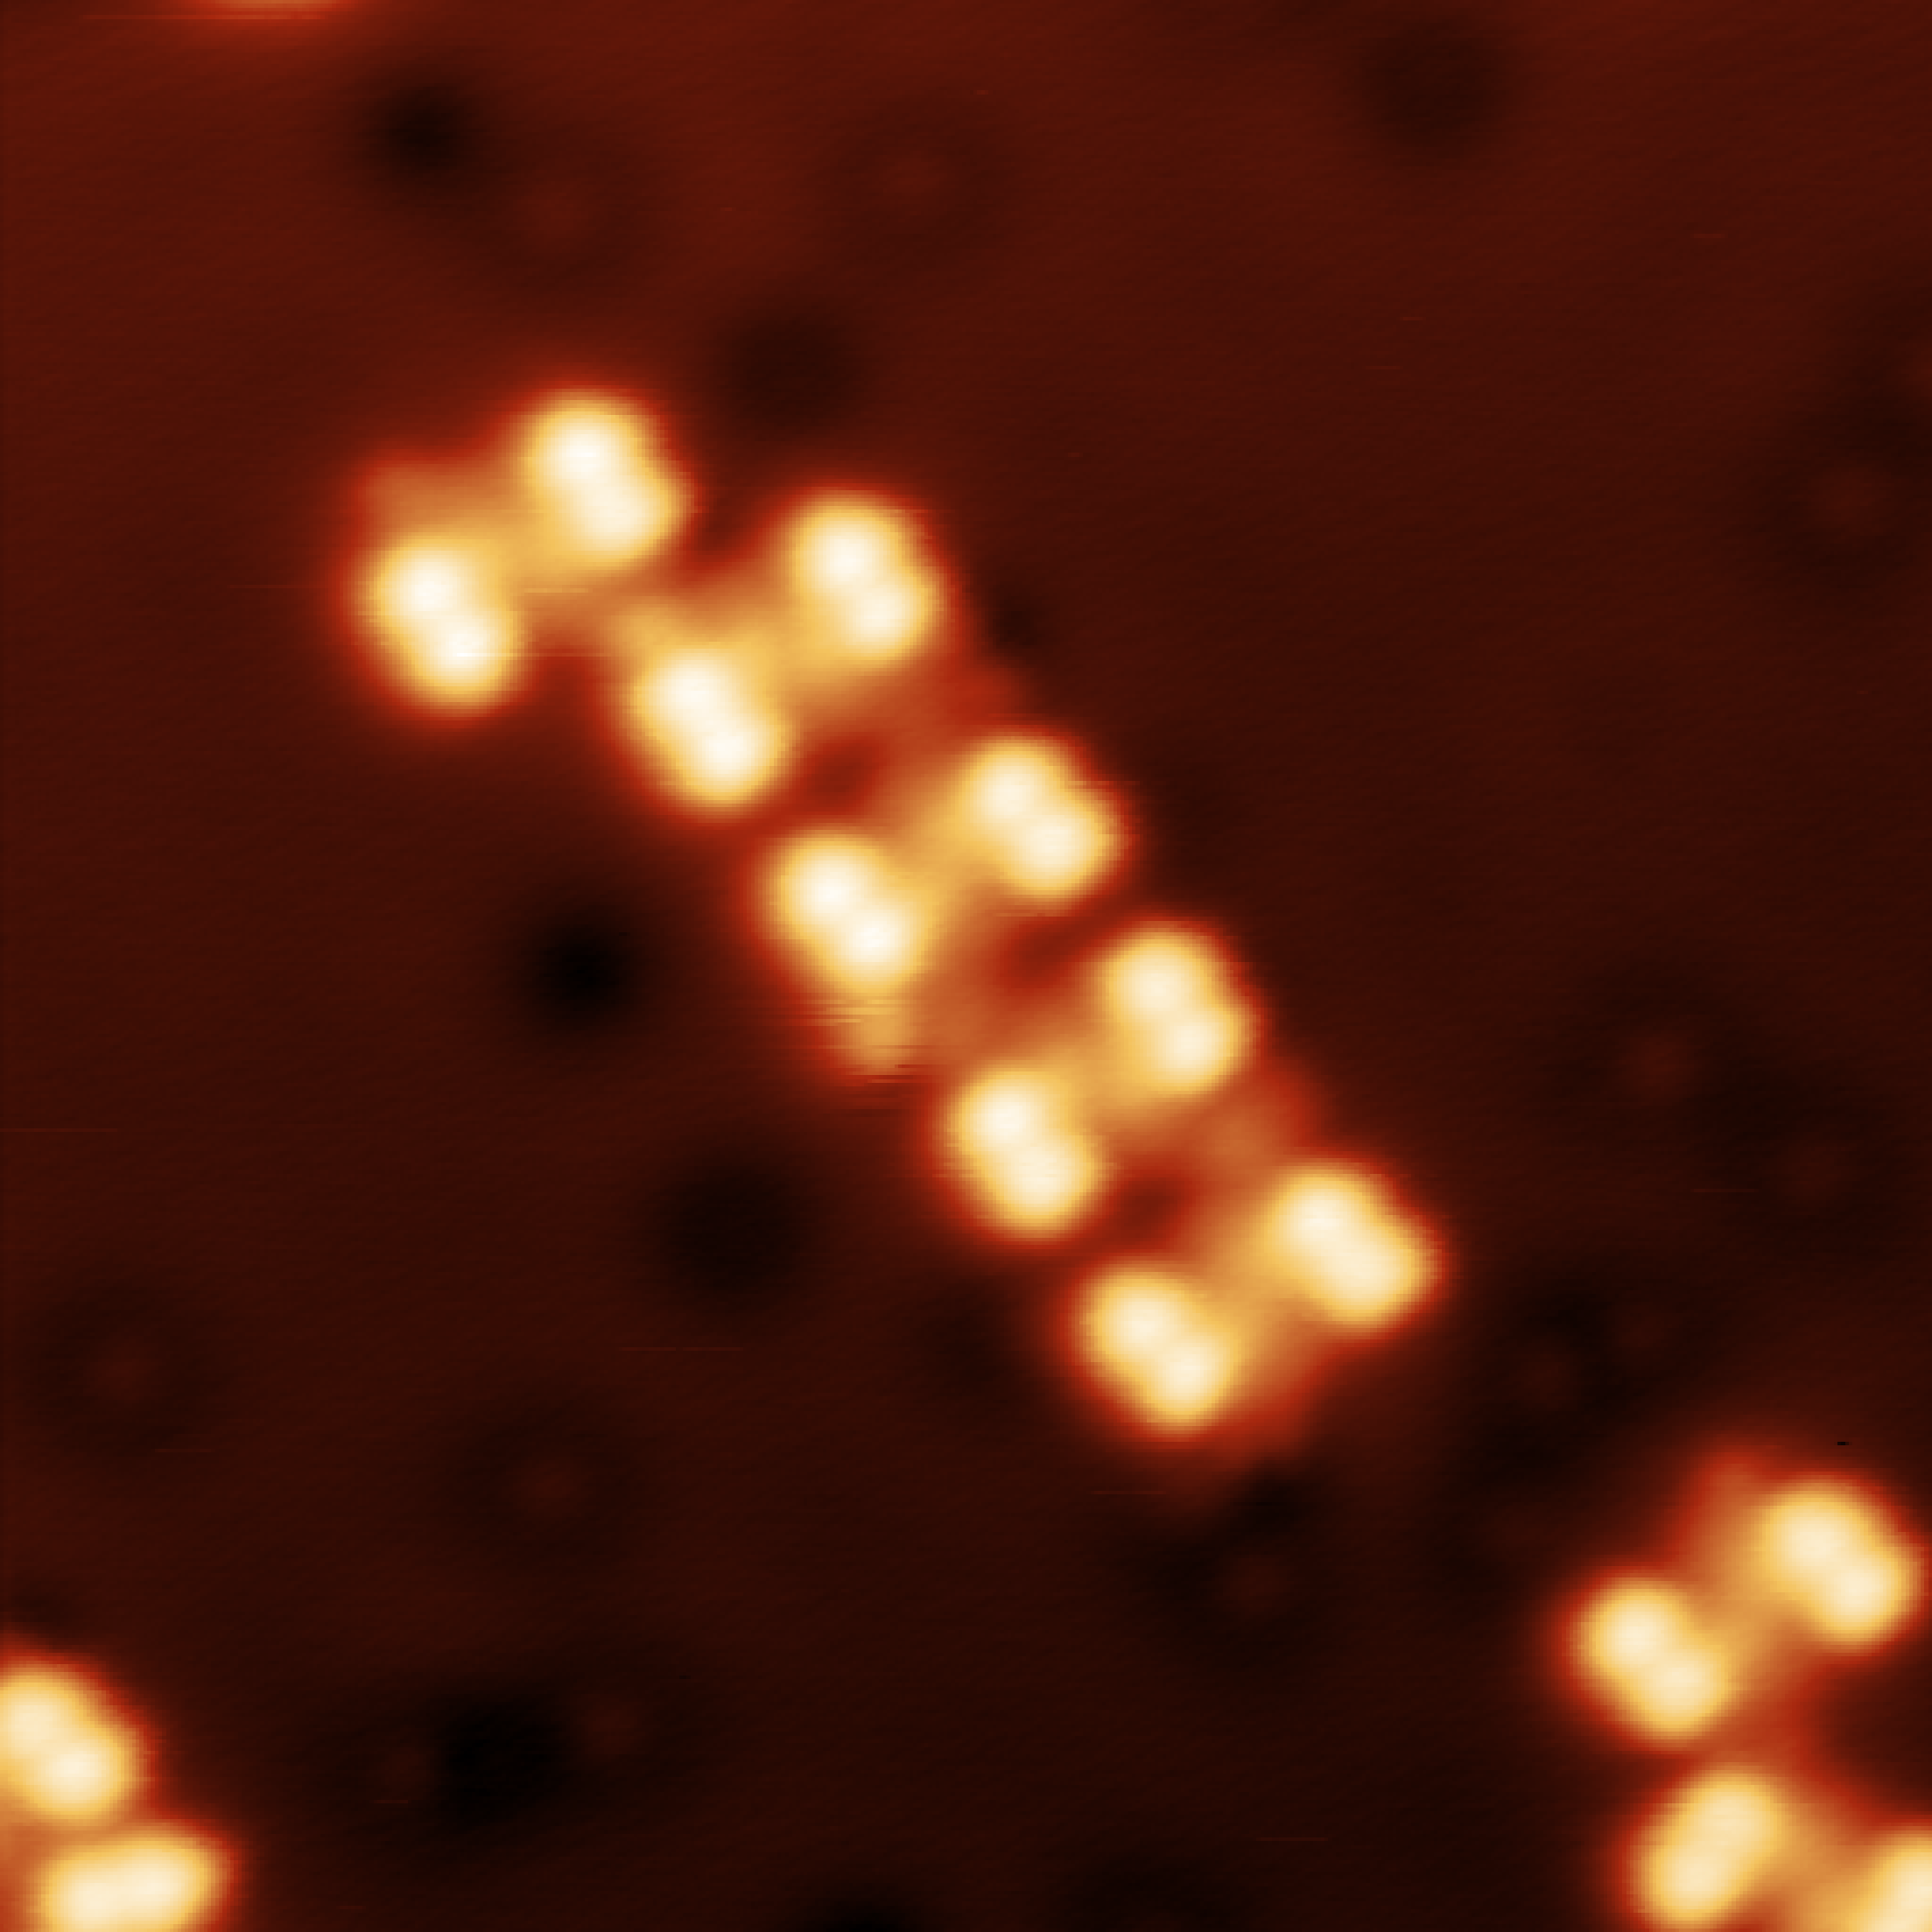
\includegraphics[width=0.45\textwidth]{./images/F160427-154618-R}
			\label{trans-nitro-on-cu111-70-straight-chain}} \qquad
		\subfigure[Shited offset chain, interrupted by a kink]{
			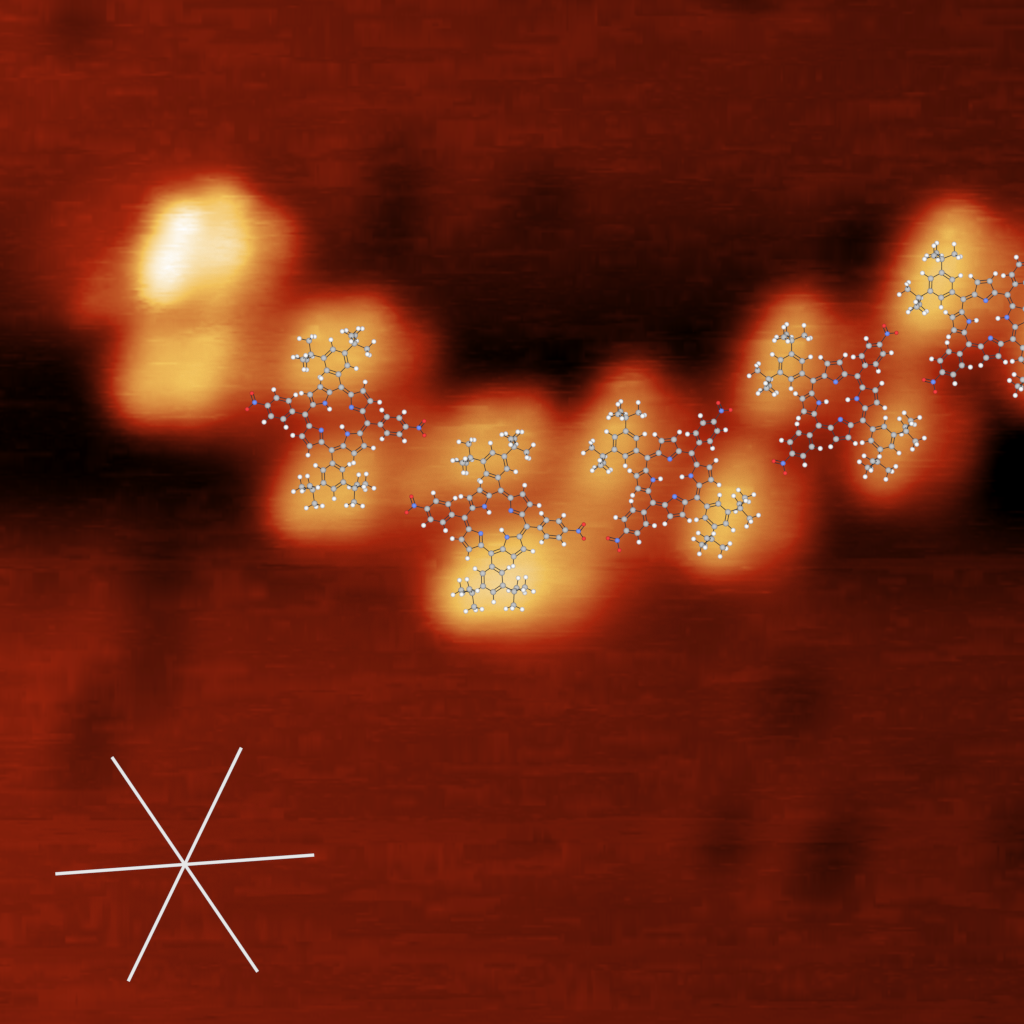
\includegraphics[width=0.45\textwidth]{./images/trans-nitro-on-cu111-120.png}
			\label{trans-nitro-on-cu111-70-shifted-chain}}
		\caption{All motifs exist at every temperature, although the chain length increases with temperature. It also looks like the chains are getting more offset- and kinked-like chains than at lower temperatures.}
		\label{fig:two-leg-trans-cu111-motifs}
	\end{figure}
	
	\begin{figure}[h]
		\centering
		\begin{minipage}{0.45\textwidth}
			\subfigure[]{
				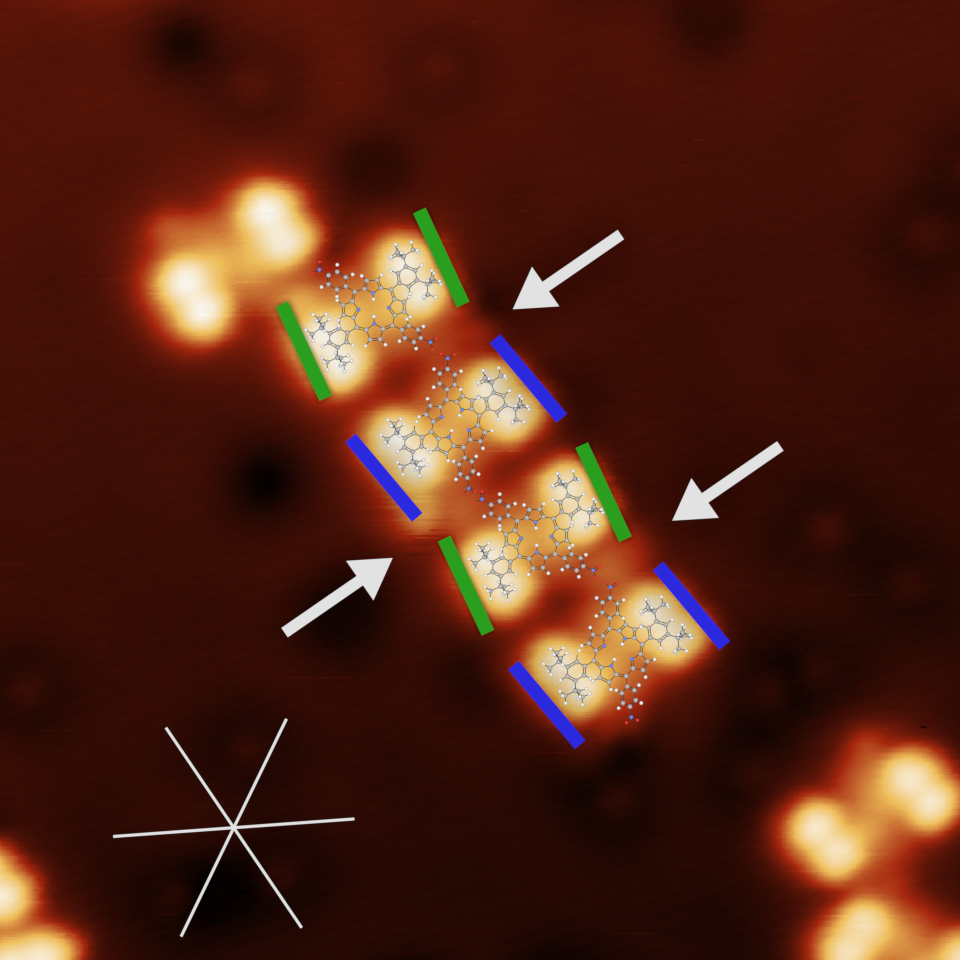
\includegraphics[width=\textwidth]{./images/F160427-154618-R-model}
				\label{trans-nitro-on-cu111-70-straight-chain-II}
			}
		\end{minipage}
		\begin{minipage}{0.45\textwidth}
			\subfigure[]{
				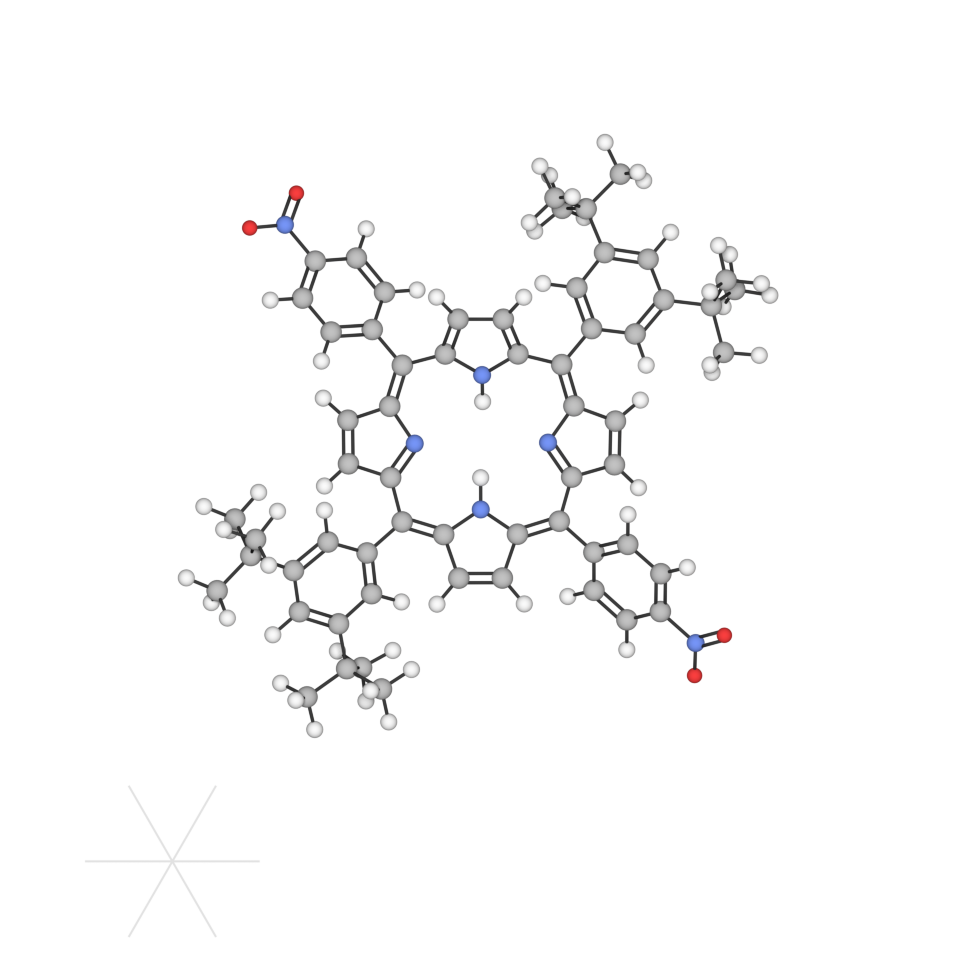
\includegraphics[width=0.45\textwidth]{./images/F160427-154618-R-gas-phase-top}
				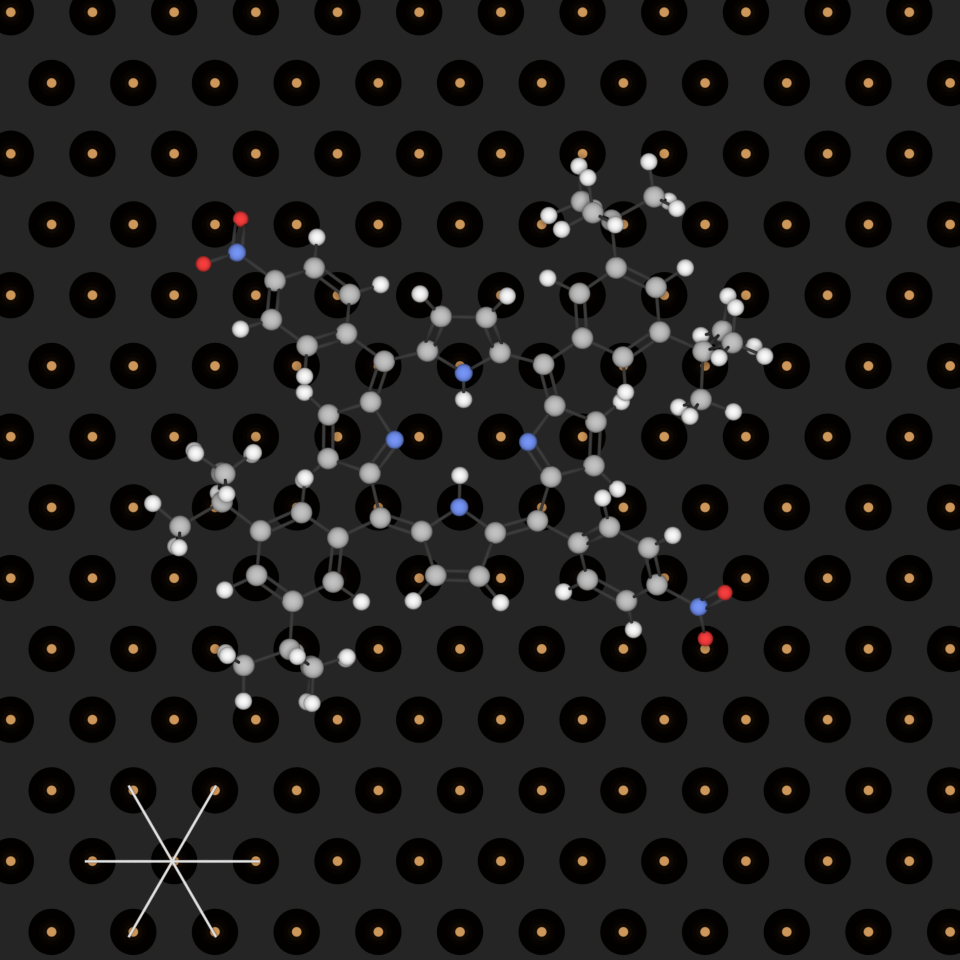
\includegraphics[width=0.45\textwidth]{./images/F160427-154618-R-cu111-top}
				\label{trans-nitro-on-cu111-70-shifted-chain-top-views}
			}
			\subfigure[]{
				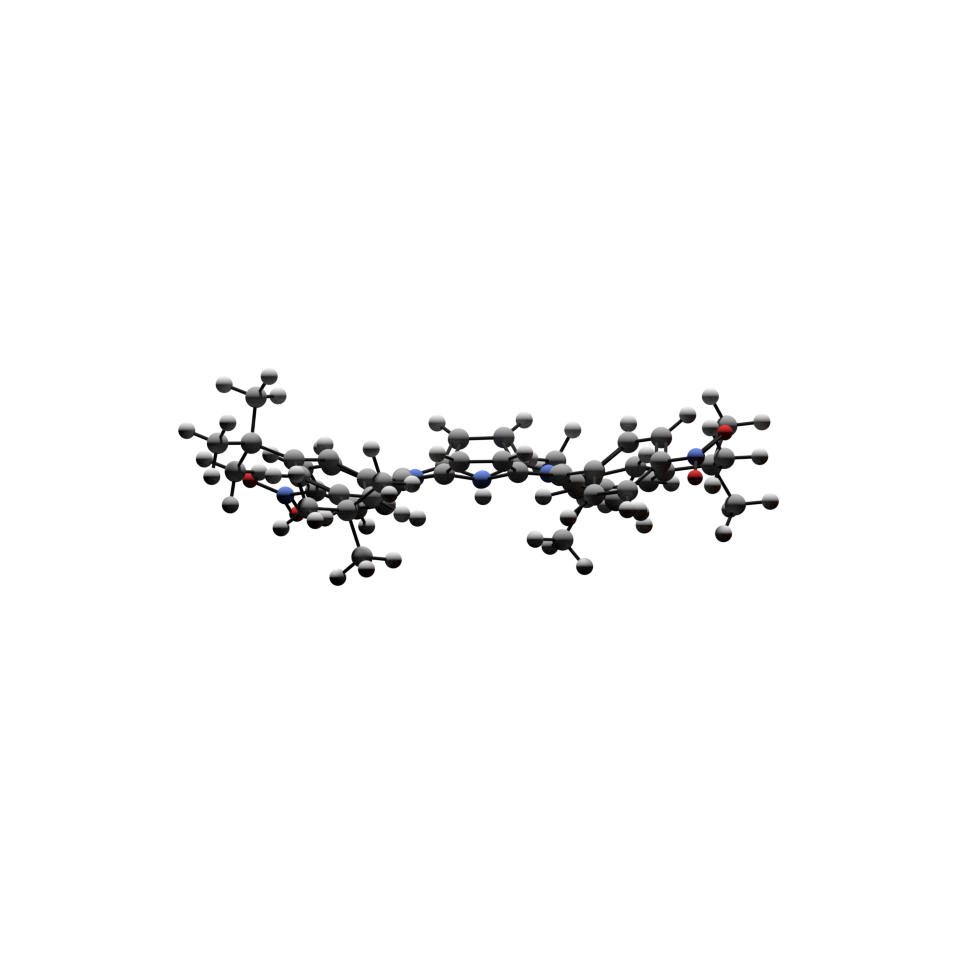
\includegraphics[width=0.45\textwidth]{./images/F160427-154618-R-gas-phase-side}
				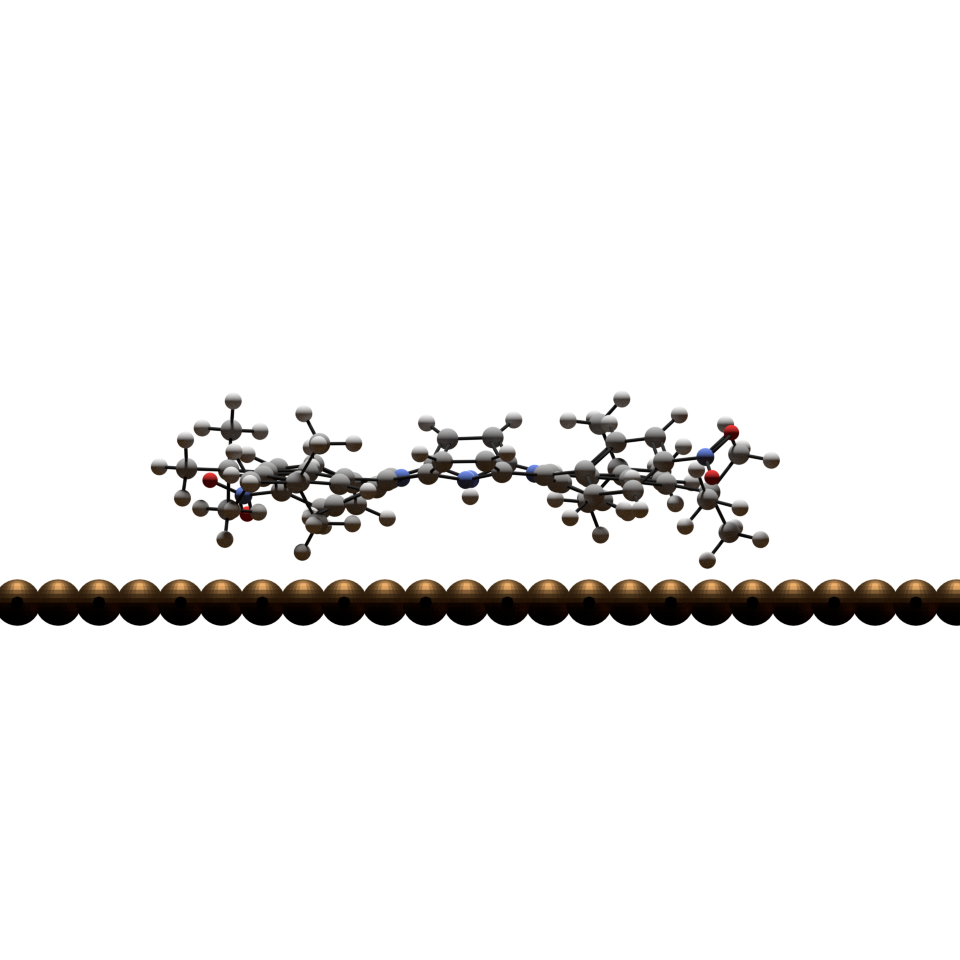
\includegraphics[width=0.45\textwidth]{./images/F160427-154618-R-cu111-side}
				\label{trans-nitro-on-cu111-70-shifted-chain-side-views}
			}
		\end{minipage}
		\caption{Straight chain binding motif on Cu(111). \subref{trans-nitro-on-cu111-70-straight-chain-II} shows an STM image together with the dense packed row indication of the substrate (white lines). Colored bars indicate the rotation of the di-tert-butyl-groups. Arrows point at places where ad-atoms are considred.
			\subref{trans-nitro-on-cu111-70-shifted-chain-top-views} Top views (\SI{6}{\nano \meter} wide) showing the molecules geometry in gas-phase (left) and after adsorption and assembly (right). Although the exact adsorption site is not known, it is considered to by on a bridge site as for 2H-P/Cu(111).
			\subref{trans-nitro-on-cu111-70-shifted-chain-side-views} Side views of above shown configurations.
		}
		\label{fig:two-leg-trans-cu111-motifs-1}
	\end{figure}
	
	During modeling \autoref{fig:two-leg-trans-cu111-motifs-1} several points became clear. 
	\begin{itemize}
		\item First consider the even apparent height of the di-tert-butyl groups. It indicates that both groups in a legs have comparable heights and it is likely that the phenyl ring bearing these groups is rotated for an even alignment of the tert-butyl groups with regard to the substrate level.
		\item Orientation of di-tert-butyl phenyl groups is the same within a single molecule but alternates (by $\approx \SI{10}{\degree}$) in neighboring molecules in a chain. This is indicated by blue and green lines in \autoref{trans-nitro-on-cu111-70-straight-chain}, each representing a common orientation.
		\item Second the minor contrast variations in the central porphine core change as the orientation of the di-tert-butyl-groups. Free base porphine core is likely to adsorb with its axis  - formed by opposing nitrogens in the core - aligned parallel to the dense packed crystal direction\cite{rojas_surface_2012}. In the present case, the molecule is lifted from the substrate by the bulky di-tert-butyl groups. Hence the porphine core interaction with the crystal substrate is considerable lower than in the 2H-P case. Still, every second molecule has the same orientation, while neighboring molecules are rotated by \SI{30}{\degree}.
		\item The gap between di-tert-butyl-phenyl groups of neighboring molecules is larger on one side of the chain than on the other and shows a larger apparent height (white arrows in \autoref{trans-nitro-on-cu111-70-straight-chain}). Although identification of surface ad-atoms is not straightforward with an STM, they are believed to originate from the copper surface.
	\end{itemize} 
	The best fitting model consists of molecules with a center-center distance of \SI{1.9 \pm 0.1}{\nano \meter}
	
	Having a closer look to the nitro groups, one recognizes a close proximity of these to each other. Also note the light protrusions in between two adjacent molecules' butyl groups (adatom?). If the legs are rotated by just \SI{15}{\degree}, the nitro groups would point to these protrusions. This rotation costs not much energy and is about \SI{25}{\kilo\J/per\mol} \textcolor{red}{\textbf{(( please cite something, value is for rotated phenyl ring at a porphine core I guess ))}}. Considering these protrusions as Cu-ad atoms (already occurred in chapter \ref{chapter:TPCN-adatoms} as protrusions in between TPCN chains which may change their position in discrete position in the molecule.) This Cu-ad atom may direct the binding of the nitro groups towards it, making them bend outwards. The position of the cooper atom itself may rely on its registry to the substrate - preferring a threefold coordination site as known for copper  \textcolor{red}{\textbf{(( citation ))}}.
	
	The second motif is a chain motif, too. Orientation of molecular axis and dense packed substrate atom rows are the same and again the di-tert-butyl groups orient along them. The difference is a lateral offset between the molecules to shift each of them by half a molecules width. The center-center distances are \SI{1.9 \pm 0.1}{\nano \meter}. It is harder to quantify a possible orientation of the nitro-phenyl groups, since as well straight as well as bended configurations match the assembly. In this binding motif, stable connections between molecules are most likely due to nitro-phenyl groups pointing to di-tert-butyl groups and therefor stabilizing the assembly.
	
	\subsection{on Ag(100)}
	% TBP-double-Ag100
	\paragraph{Unit cell}
	When adsorbed on a square (100) silver surface, the molecules interestingly arrange in a trihexagonal tiling (see figure \ref{fig:two-leg-trans-ag100-motif}). The molecules at the perimeter of this island is nicely distinguishable and continuing their regular pattern to the center of the island results in an accurate description of the assembly. The unit cell is determined to be $\underline{\qquad \qquad}$ and the hexagonal unit cell is shown in \autoref{fig:two-leg-trans-ag100-unit-cell}, bearing three molecules.\footnote{Similar open porous network can be created, e.g. cyano functionalized triarylamines on Au(111) \cite{gottardi_cyano-functionalized_2014}.}
	
	\paragraph{Molecular orientation}
	The molecules are arranged so that each molecule has one of its di-tert-butyl-groups in one hexagonal pores and the other in the neighboring one. Each pore is made up of six molecules arranged on a hexagon with $\underline{\qquad \qquad}$ long edges. Each vertex is occupied by a single molecule, neighboring molecules on the hexagon are rotated by \SI{60}{\degree}. The pores are created by free space where the di-tert-butyl-groups point towards each other. The nitro-phenyl groups point towards the intermediate space where smaller triangular openings are formed. At their edges the nitro-phenyl groups connect to the neighboring di-tert-butyl groups.
	
	Considering a former orientation calibration on Ag(100) where the direction of the dense packed crystal direction was determined, the orientation with regard to the substrate is given as white lines in \autoref{fig:two-leg-trans-ag100-unit-cell}: The long and short axis of the unit cell (marked as green cross in \subref{fig:two-leg-trans-ag100-unit-cell}) is almost collinear, just differing by less than \SI{10}{\degree}. Since the calibration was done with another preparation the angle calibration may not be \SI{100}{\percent} accurate because the sample was moved in the meantime. That may result in an little angle uncertainty. Please see  \autoref{F160429-185245-R-model-2-crystal-orientation.png} in \fullref{appendix:TBP} for a detailed image.
	
	\paragraph{Contrast within single molecule}
	A closer look to the geometries in high resolution STM data gives clue to the rotation of the di-tert-butyl-groups and is visualized in \autoref{fig:two-leg-trans-ag100-single-molecule}. Focusing on the STM contrast of a single molecule, one can see that it is dominated by the di-tert-butyl-groups on both sides of the molecule. These look like small triangles in the STM with a single brighter protrusion enclosed by the footprint. The bright protrusion is never on the same side of the triangular footprint thus the di-tert-butyl-groups are believed to be rotated in two different directions - lifting opposite parts of the functional group.
	\begin{figure}[]
		\centering
		\subfigure[STM topography of several molecular islands grown next to a step edge. Areas with trihexagonal tiling as well as some domain boundaries are visible.]{
			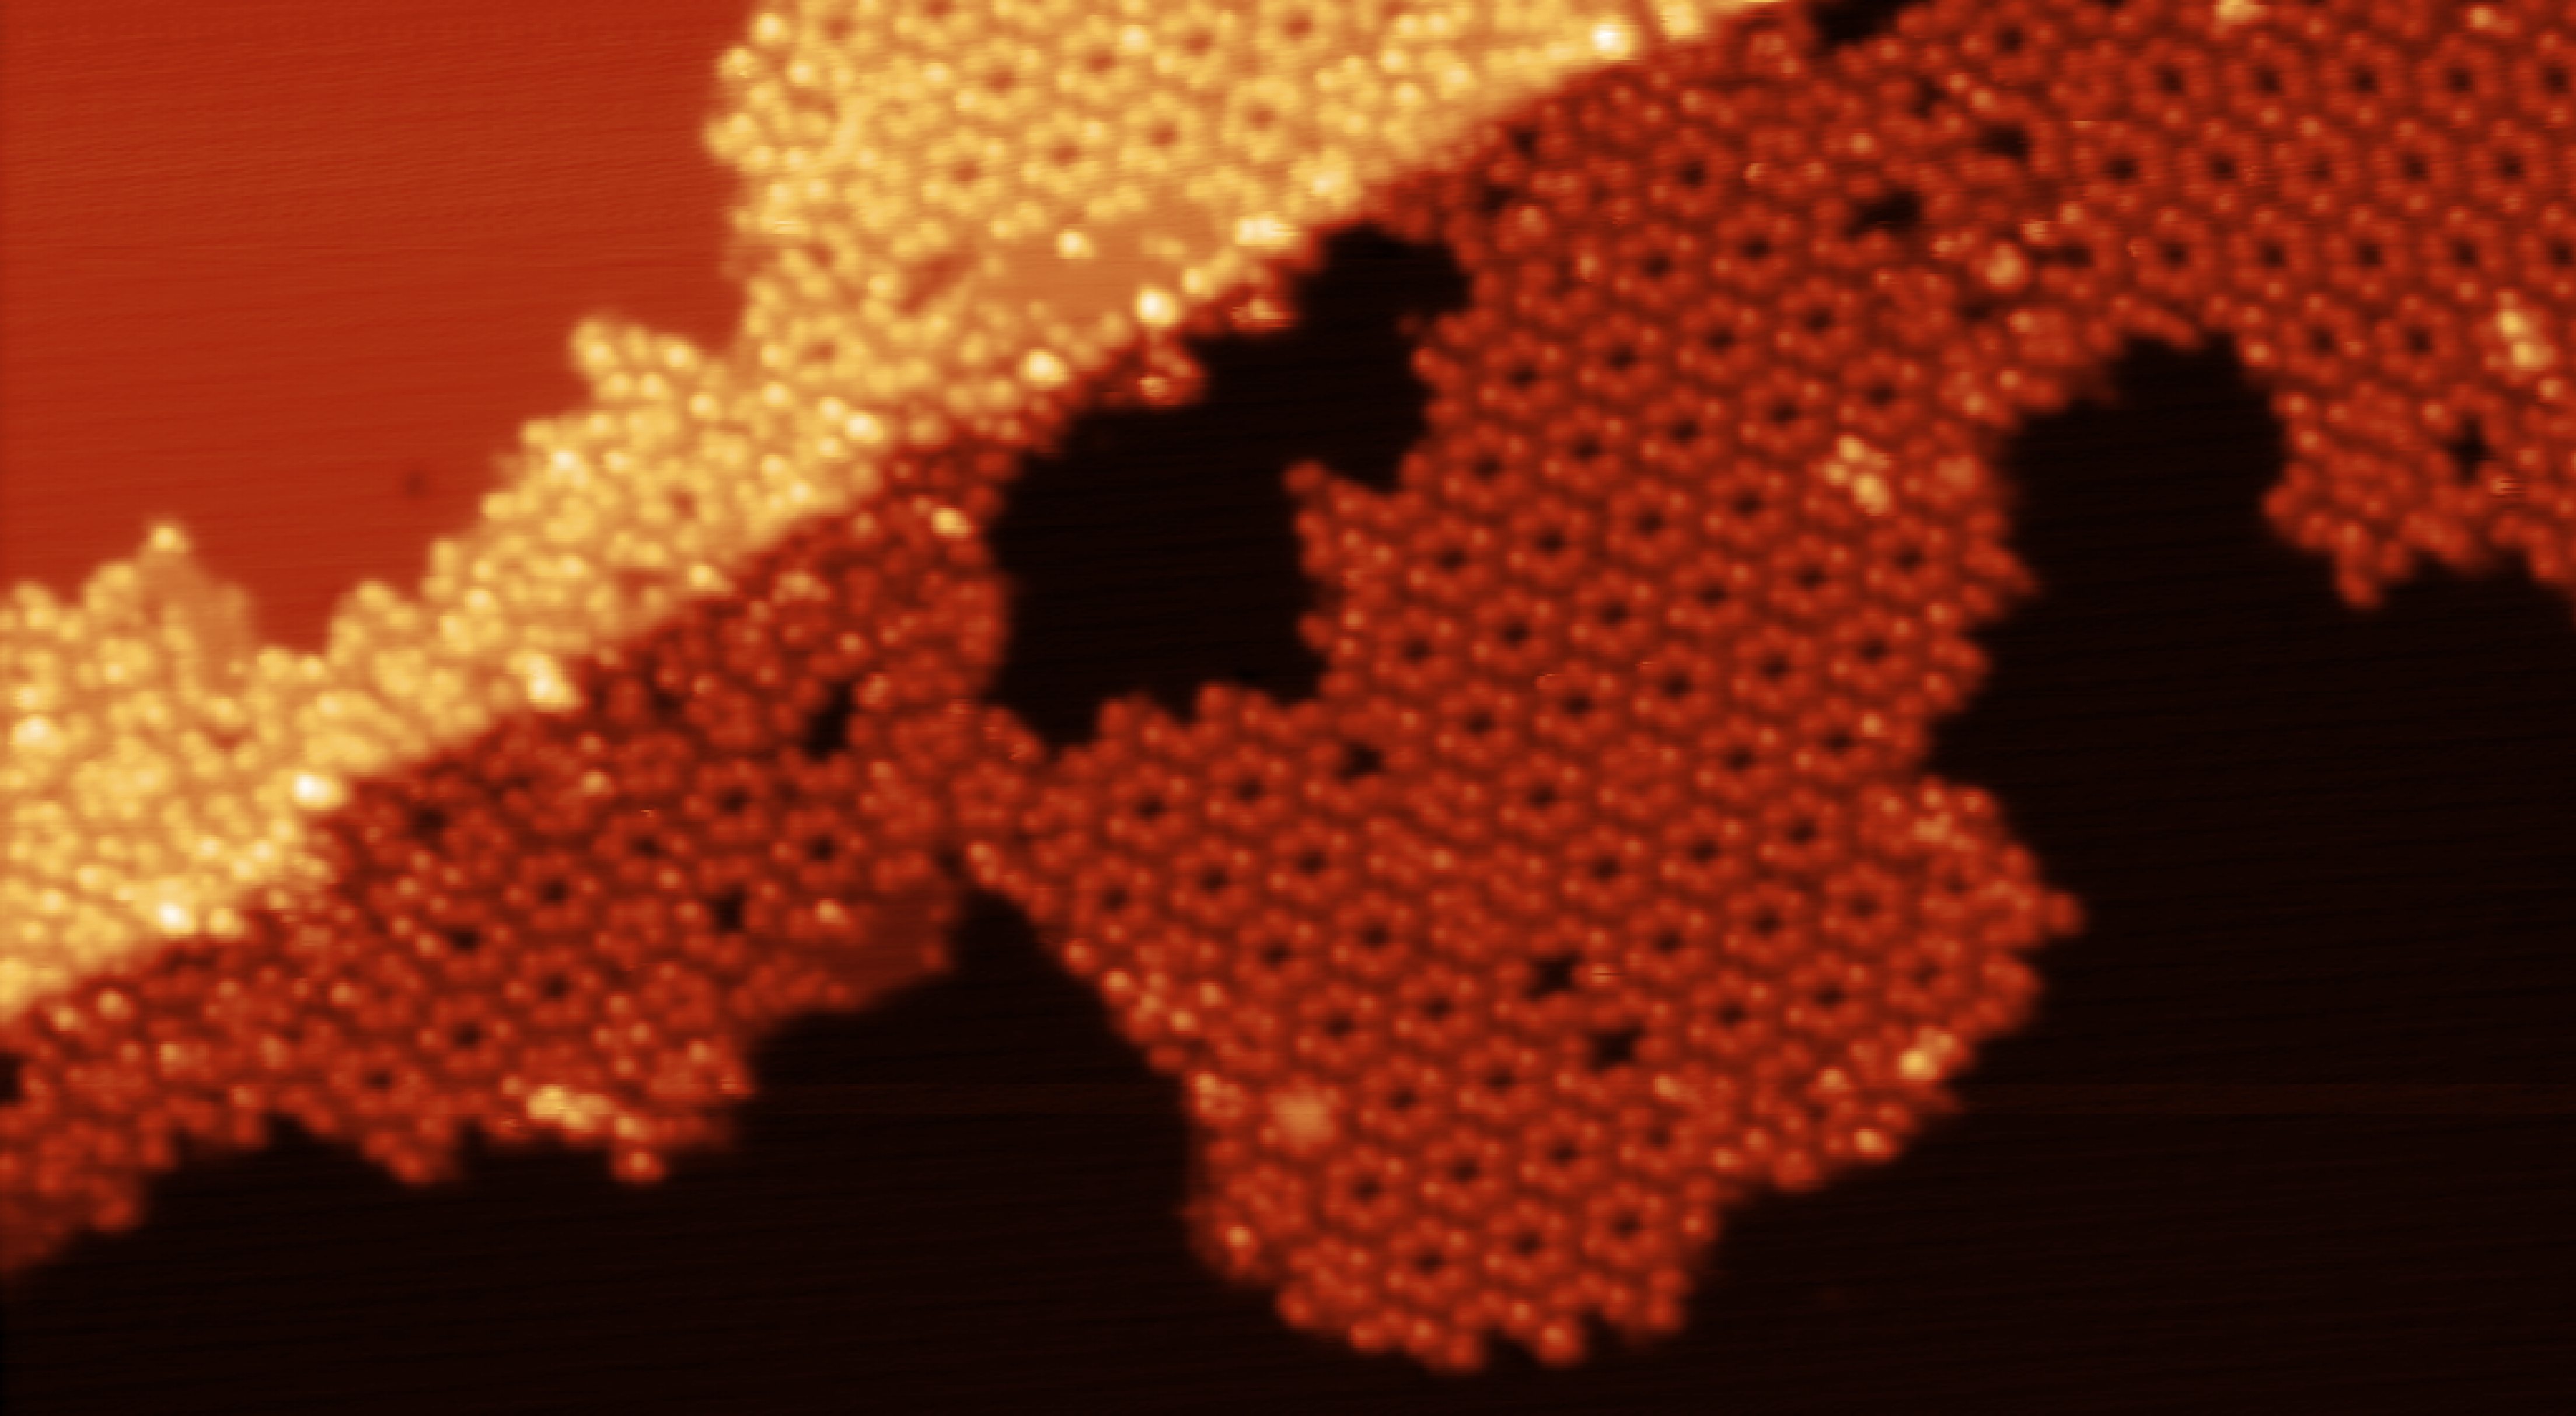
\includegraphics[width=\textwidth]{./images/F160429-172019}
			\label{fig:two-leg-trans-ag100-overview}
		} %COARSE MODE!
		\subfigure[Hexygonal unit cell with overlaid molecular models.]{
			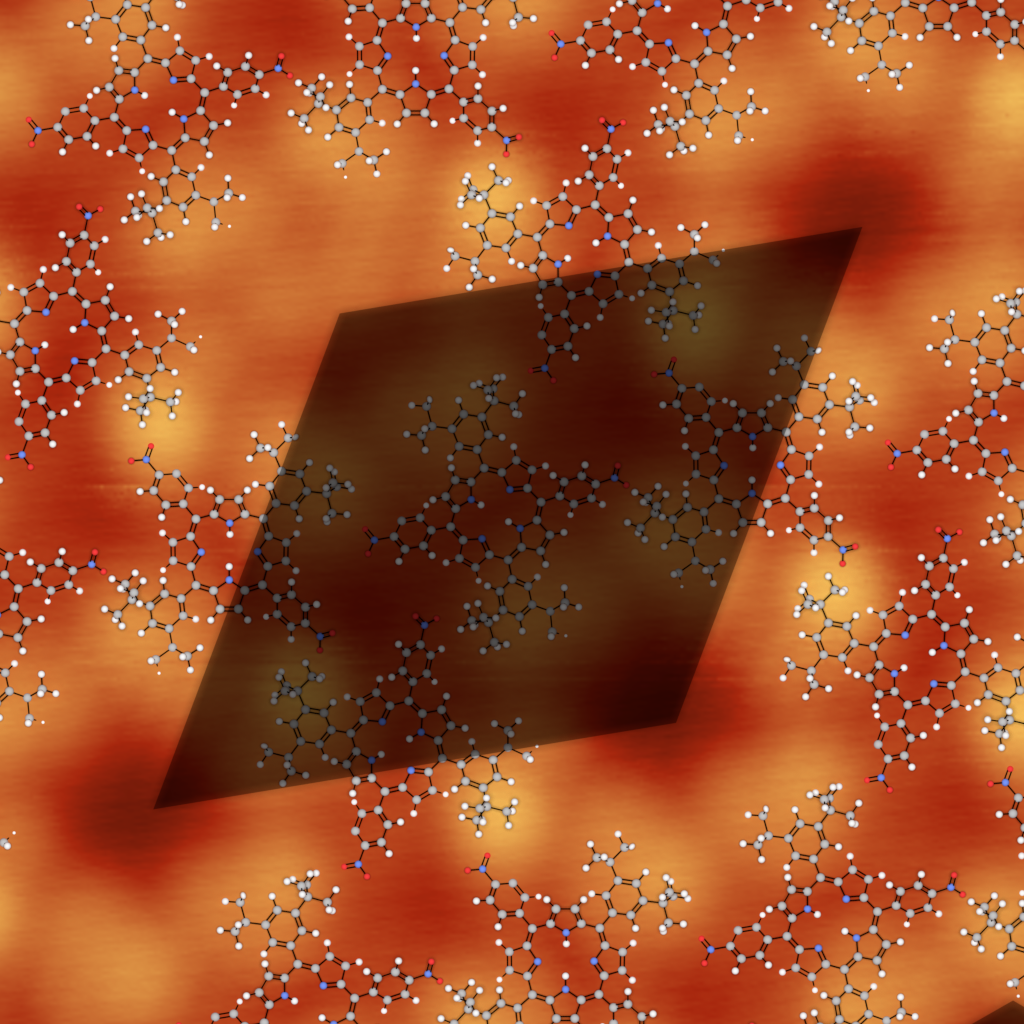
\includegraphics[width=0.3\textwidth]{./images/F160429-185245-R-model}
			\label{fig:two-leg-trans-ag100-unit-cell}
		} \quad %COARSE MODE!
		\subfigure[Enlarged view on the molecules rotated di-tert-butyl-group and highest elements enclosed by brighter circles..]{
			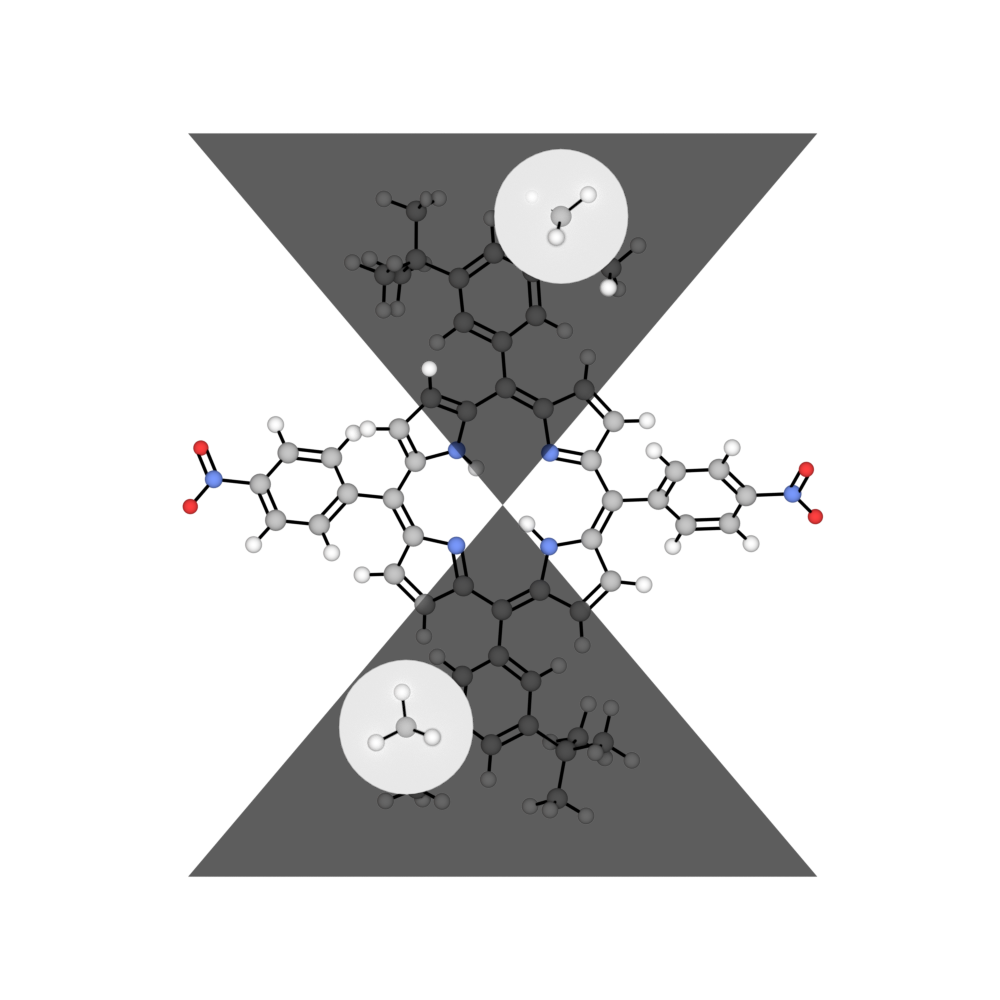
\includegraphics[width=0.3\textwidth]{./images/F160429-185245-R-single-molecule}
			\label{fig:two-leg-trans-ag100-single-molecule}
		} %COARSE MODE!
		\caption{Trans-TBP adsorped on Ag(100) at room temperature. \subref{fig:two-leg-trans-ag100-overview} shows a large overview of the assembled molecules. The unit cell constituents are enlarged in \subref{fig:two-leg-trans-ag100-unit-cell} where parts of \subref{fig:two-leg-trans-ag100-overview} are shown with molecular models overlaid. \subref{fig:two-leg-trans-ag100-single-molecule} shows a single molecule crossing a horizontal plain to emphasize high lying part in the molecule that are marked with white circles and will appear brighter in STM. All images recorded with \SI{437}{\milli\volt}, \SI{0.1}{\nano\ampere}, color scale \SIrange{0}{650}{\pico\meter}
		}
		\label{fig:two-leg-trans-ag100-motif}
	\end{figure}
	
	\paragraph{Domain boundaries}
	The observed domain boundaries are imaged in \autoref{fig:two-leg-trans-ag100-domain-boundary}. On both sides the regular tiling is proceeded, but both are shifted with respect to each other by $\underline{\qquad \qquad}$. This offset results in the wrong alignment of molecules from one  domain with respect to the other domain and a discontinued growth. The resulting free area at the domain boundary is occupied by molecules from one domain that bear the wrong orientation the proceed the growth of the second domain and vice versa. This can be nicely seen in 		\autoref{fig:two-leg-trans-ag100-domain-molecular-model}, where the misalignment of one domain (left) with respect to the other (right) causes two cavities to open up between the two (lower image part). While these two are unoccupied and reveal the substrate, another type of cavity can be formed directly seen on top of the two aforementioned. Here the cavity is filled with a single molecule so that both di-tert-butyl groups interlock with the open cavity. Some is the assembly pores are filled, too. Here the space of the pore prohibits a complete molecule to fit in, the observed adsorbates in the pores are attributed to molecular fragments like tert-butyl-groups that were incorporated by the assembly during the island growth.
	
	\begin{figure}[]
		\centering
		\subfigure[Domain boundary]{
			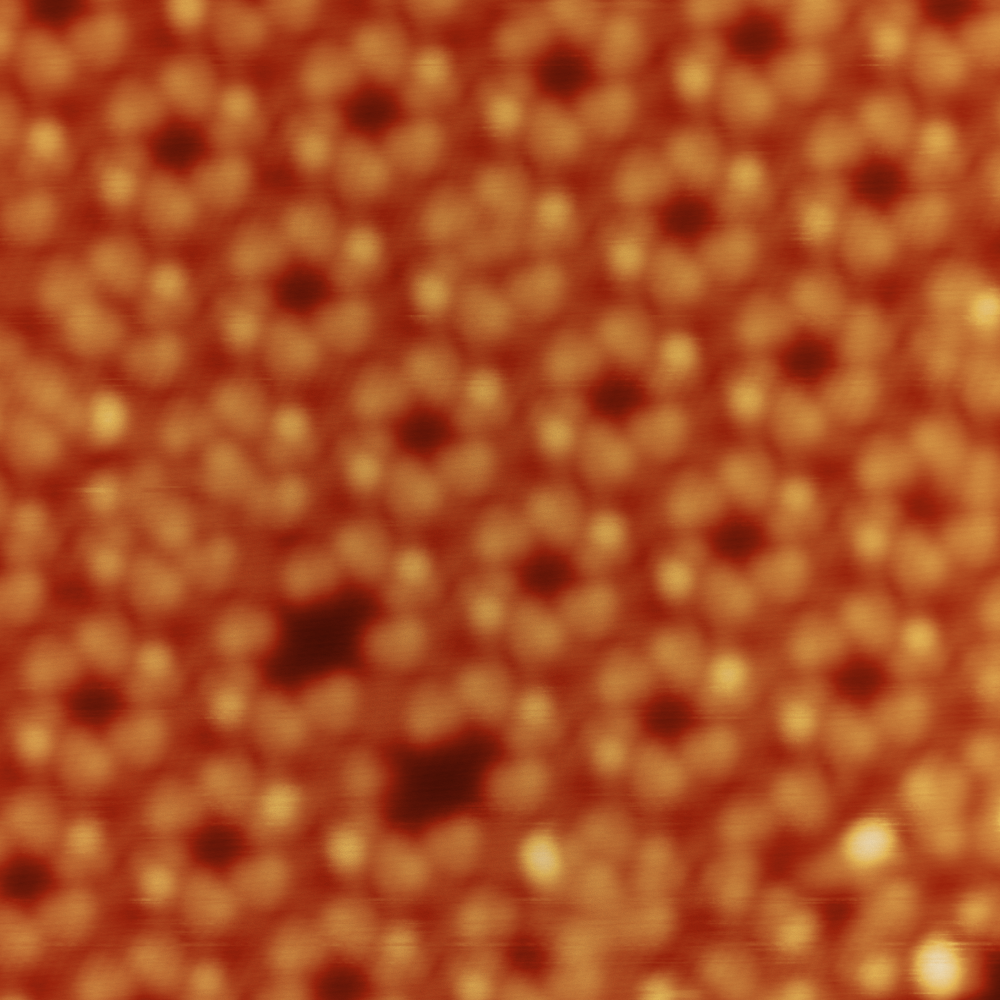
\includegraphics[width=0.35\textwidth]{./images/F160429-185245-R--2}
			\label{fig:two-leg-trans-ag100-domain-overview}
		} %COARSE MODE!
		\subfigure[Model representation of domain boundary]{
			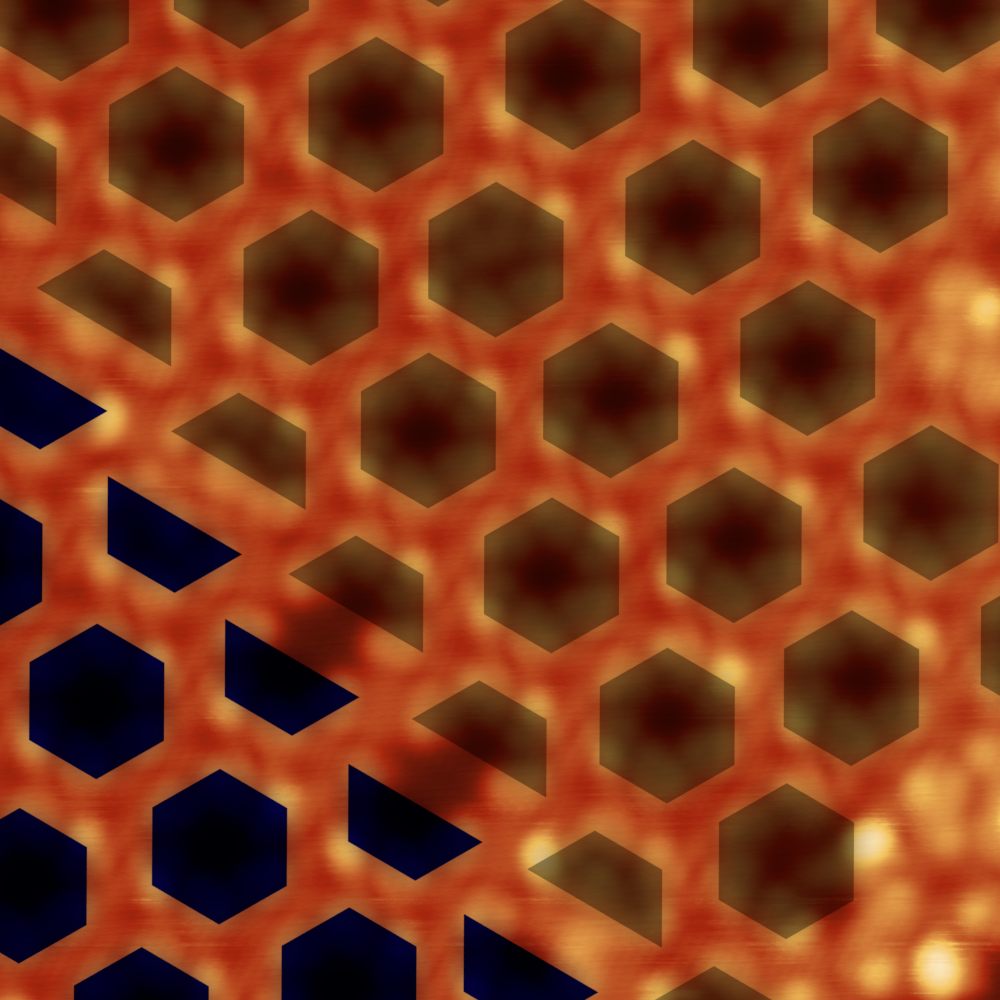
\includegraphics[width=0.35\textwidth]{./images/F160429-185245-R--2-model}
			\label{fig:two-leg-trans-ag100-domain-model}
		} %COARSE MODE!
		\subfigure[Molecular model of domain boundary, overlaid with two unit cells]{
			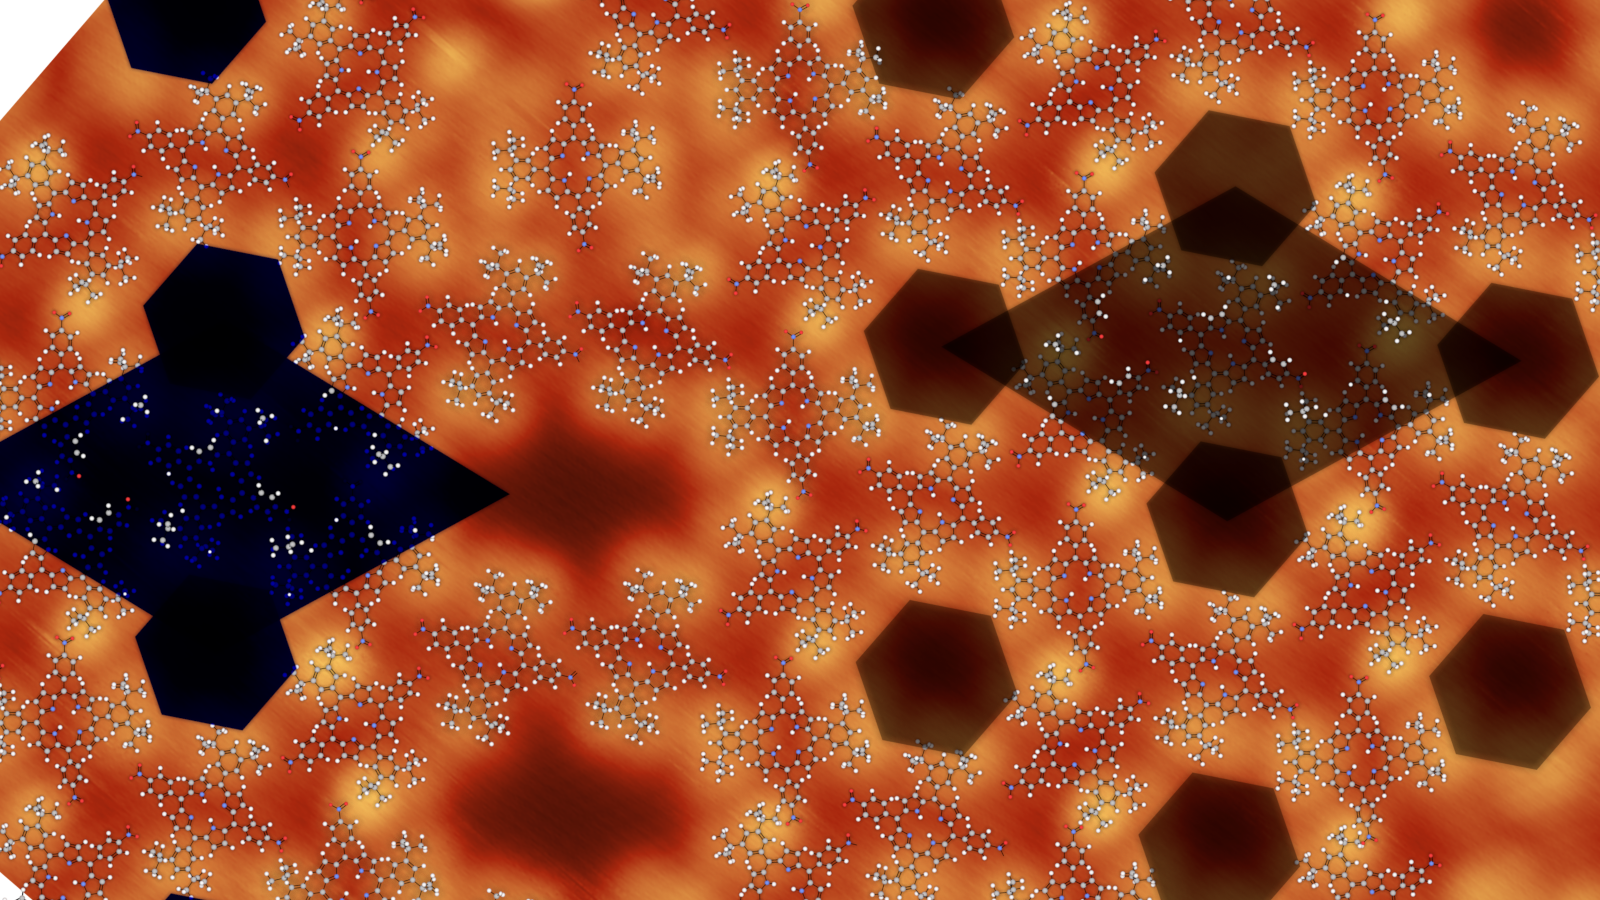
\includegraphics[width=0.7\textwidth]{./images/F160429-185245-R--domain-overview}
			\label{fig:two-leg-trans-ag100-domain-molecular-model}
		} \quad %COARSE MODE!
		\caption{Domain boundary of trans-TBP adsorbed on Ag(100) at RT. \subref{fig:two-leg-trans-ag100-domain-overview} shows an overview of the domain boundary together with its model representation in \subref{fig:two-leg-trans-ag100-domain-model}. The assembly close by is modeled in \subref{fig:two-leg-trans-ag100-domain-molecular-model} where a rotated detail view of \subref{fig:two-leg-trans-ag100-domain-overview} is shown and molecular models overlaid. All images recorded with \SI{1.3}{\volt}, \SI{0.1}{\nano\ampere}, color scale \SIrange{0}{650}{\pico\meter}
		}
		\label{fig:two-leg-trans-ag100-domain-boundary}
	\end{figure}

\section{Summary \& Discussion}
\textcolor{red}{\textbf{TEXT}}
	
\section{Conclusion}
\textcolor{red}{\textbf{
		The driving force for orienting the whole molecule on the surface remains speculative. On Ag(100), neither an orientation of the molecules main axis with respect to the substrate, nor a orientation of butyl-groups along the dense packed substrate rows can be seen - which again favors Cu-substrate interactions as dominant role.
		When the copper is exchanged with silver to act as substrate, TBP behaves quite different. Although the distribution is homogeneous on the surface, the interaction between molecules look different. While on copper the most abundant binding motif is the head-to-head dimer, this motif does not appear on silver as often as on copper. Two other motifs emerge on silver.
		The interaction between the butyl-phenyl groups is considered to be van der Waals like \cite{iacovita_controlling_2012}, stabilizing the conglomerate.
	}}
	
	